\documentclass[a4paper,11pt]{article}

%%% ---------------- %%%
%%% --- Packages --- %%%
%%% ---------------- %%%
    \usepackage{graphicx}
    \usepackage[utf8]{inputenc}
    %\usepackage{amsmath}  % for the align environment 
 %   \usepackage{authblk}
 %   \usepackage[space]{grffile}
 %   \usepackage{latexsym}
%    \usepackage{textcomp}
%    \usepackage{longtable}
%    \usepackage{tabulary}
   % \usepackage{booktabs,array,multirow}
   % \usepackage{amsfonts,amsmath,amssymb}
 %   \usepackage[table]{xcolor}
%    \definecolor{lightgray}{gray}{0.9}
 %   \definecolor{lightergray}{gray}{0.7}
  %  \usepackage{colortbl}
 %   \usepackage{caption} % for individual caption (S in Appendix) 
    
   % \usepackage{lineno}         % for line numbers 
   % \usepackage{mathptmx}       % Times new Roman 1
   % \usepackage[T1]{fontenc}    % Times new Roman 2
   % \usepackage{subcaption}     % subfigure environment
   % \usepackage[labelfont=bf]{caption} % Labels dick gedruckt
   % \usepackage[font=small]{caption}  % caption text body small   
    \usepackage{natbib}         % for citations
     \usepackage[a4paper, left = 2.5cm, right = 2.5cm, top = 2.5cm, bottom = 2.5cm]{geometry}            % page layout
    \usepackage{setspace}       % line spacing

  %  \usepackage{hyperref}
  %\usepackage{microtype}          % to avoid over- or underfull hboxes 
    

    
%%% ---------------- %%%
%%% --- Settings --- %%%
%%% ---------------- %%%

\doublespacing      % double spaced

\begin{document}

\title{Should ecologists prefer model- over algorithm-based multivariate methods?}

\author{Jonathan F. Jupke and Ralf B. Schäfer \\ iES Landau, Institute for Environmental Sciences,\\ University Koblenz-Landau, Fortstraße 7, 76829 Landau, Germany}

%%% ----------------- %%%
%%% ---Title Page --- %%%
%%% ----------------- %%%

    \maketitle
    corresponding Author: Jonathan F. Jupke, jonathanfrederik@aol.com,
    +49 06341 280-33285\\


    \newpage
    %%% ---------------- %%%
    %%% --- Abstract --- %%%
    %%% ---------------- %%%

        \begin{abstract}%  Less than 250 words 
        %motivation 
            Ecological data sets often record the abundance of several species, together with a set of explanatory variables. 
            %
            Multivariate statistical methods are optimal to analyze such data and are thus frequently used in ecology for exploration, visualization, and inference. 
            %
            Most of the common approaches are algorithmic, they follow mathematical routines like correspondence - or distance-based analyses, which stands in stark contrast to univariate statistics, where data models, assuming specific distributions, are the norm.
            %
            However, through advances in statistical theory and computational power, models for multivariate data have gained traction. 
            %
        %problem statement
            Systematic and simulation-based performance evaluations of these methods are important as guides for practitioners but still lacking.
        %approach
            Here, we compare two model-based methods, multivariate Generalized Linear Models (MvGLM) and Constrained Quadratic Ordination (CQO), with two algorithm-based methods, distance-based redundancy analysis (dbRDA) and Canonical Correspondence Analysis (CCA).
            % 		
            We studied the performance of the methods to discriminate between causal variables and noise variables for 180 simulated data sets covering different sample sizes and data distributions.
        %results
            MvGLM and dbRDA differentiated accurately between causal and noise variables.
            %
            The former had the lowest false positive rate (0.008) while the latter had the lowest false negative rate (0.017).
            %CCA
            CQO and CCA had the highest false negative rate (0.291) and false positive rate (0.256), respectively. 
        %conclusions
          Our study shows that both model- and algorithm-based methods have their place in the ecologists statistical toolbox. 
          % 
        MvGLM and dbRDA are reliable for analyzing species-environment relations, whereas both CQO and CCA exhibited considerable flaws, especially with linear environmental gradients. 
          %
           
        \end{abstract}

%     %%% ----------------- %%%
%     %%% --- Key-Words --- %%%
%     %%% ----------------- %%%

        {\bf Keywords:} 
        %1.
        statistical models,
        %2.
        numerical simulations,
        %3 
        ordination, 
        %4
        multivariate analysis, 
        %5
        variable selection
    \newpage

\section{Introduction}

	Which environmental gradients control species abundances and community composition, is one of the most essential questions in ecology [e.g.][]\citet{Clements1907}  and the current alteration of ecosystems at an unprecedented rate endows it with a new urgency \citep{pacifici2015assessing}. 
	%
	Given the complexity of simulating ecological systems under artificial conditions (e.g. in microcosms), monitoring the abundance or occurrence of taxa across sites with variable  environmental conditions has been one approach to tackle this question.
	%
	Related studies deliver a sites-by-species matrix $\mathbf{Y}$ containing multivariate species abundances, which is then statistically related to  a sites-by-predictor matrix $\mathbf{X}$, containing information on the environmental predictors.
	%
	From a statistical perspective, $\mathbf{Y}$ has many undesirable properties such as
	intercorrelations between variables, 
	e.g. through biotic interactions \citep{morales2015inferring},
	probability distributions other than the normal, 
	more species than sites \citep[\textit{high dimensionality}, especially in DNA barcoding studies,][]{cristescu2014barcoding},  
	and many zeros, because most species are commonly absent from most sites (\textit{sparsity}) \citep{mcgill2007species}. 
	
% 	%------------------------------%
% 	%&		Zweite Absatz:
% 	%&	Distance Based + Whats wrong with it
% 	%------------------------------%
    
    While univariate data are routinely analyzed by model-based methods like ANOVA, generalized linear models and linear mixed models, multivariate data are most often analyzed with algorithm-based methods.
    %
    Most of the latter are variations on three basic approaches: i) correspondence analysis, ii) redundancy analysis, or iii) analysis of pairwise distance matrices. 
    %
    Algorithm-based methods have weak links to ecological theory and do not take the data's statistical properties into account. 
    %
    In distance-based algorithms, for example, the researcher implicitly assumes a mean-variance relationship of the data by choosing a certain distance metric. 
	% 
	For instance, Minkowski distances (e.g. Manhattan and Euclidean) assume a constant variance across all mean values \citep{TerBraak1988}
	%
	whereas species abundances often show a quadratic mean-variance relationship \citep{routledge1991taylor, yamamura1999transformation}.
	%
	Whether a distance metric is appropriate depends on the properties of the data and the aim of the study, as each metric extracts different information from the raw data. 
	%
	The choice is complicated by the vast amount of available metrics \citep[see][]{Legendre2012}.
	%
	Misspecification of the relationship by choosing an inappropriate distance metric can lead to erroneous conclusions as demonstrated by \citet{Warton2012}.
	%
	An alternative to algorithm-based analyses that accounts for mean-variance relationships and incorporates ecological assumptions is the model-based approach.\\
 
	%------------------------------%
	%&		Dritte Absatz:
	%&	Model Based Approach
	%------------------------------%
	The model-based approach consists of explicitly specifying a statistical model of the process that generated the observed data \citep{Warton2015a}.
	%
	This includes properties such as marginal distributions, overdispersion, zero-inflation, mean-variance relationship, and correlation structure, all of which can be flexibly tailored to the data and the research question.
	%
	While this approach is ubiquitous in univariate analyses \citep[e.g.][]{bolker2008ecological, zuur2010protocol}, it has long been uncommon in multivariate ecological analyses, largely due to the absence of suitable models \citep{anderson2001new}.
	%
    However, advances in statistical theory and computation power have led to a surge of models for multivariate abundance data. 
	%
	Recent examples include Hierarchical Modeling of Species Communities \citep{Ovaskainen2017}, Generalized Joint 
	%
	Attribute Modelling \citep{Clark2017},  and multivariate Generalized Linear Models \citep[MvGLM,][]{Warton2012}.
	
	%------------------------------%
	%&		Vierte Absatz:
	%&			GLMmv
	%------------------------------%
	
	In MvGLM, a separate univariate GLM is fit to each taxon, with each model using the same predictors. 
	%
	Univariate GLMs are a flexible method and are strongly advocated for the analysis of count or occurrence data as they can handle different residual distributions and mean-variance relationships \citep{OHara2010, Warton2011, Szocs2015_b}.
	%
	Extending them to multi-species abundance data was thus a natural starting point for multivariate model-based analyses \citep{Warton2012}.
	%
	The univariate models are combined by summing their test statistics, which allows for inference on the whole community.
	%
	The use of MvGLM, facilitated by an easy-to-use implementation in R  \citep[in the \textit{mvabund} R-package, ][]{Wang2019}, has steadily increased within the ecological community. 
	%
	However, direct comparisons of MvGLM to other methods remain rare, with a few exceptions.
	% 
 	\citet{Warton2012} showed that MvGLMs, in contrast to algorithm-based methods, can differentiate between location (difference in mean) and dispersion (difference in mean-variance relationship) effects. 
 	%
	\citet{Szocs2015} found that MvGLMs performed better or similarly well in terms of statistical power than Principal Response Curves (a form of redundancy analysis) when used for the analysis of ecotoxicological semi-field studies. 
	%
	However, systematic studies of data sets with known properties are lacking and this paucity of studies hampers our capacity to make informed decisions on the selection of methods for multivariate data analysis.\\

	%------------------------------%
	%&		5. Absatz:
	%&		Aim of the Study
	%------------------------------%
	
	We compared the performance of MvGLMs to differentiate between causal and noise variables to three methods of data analysis: 
	%
	Constrained Quadratic Ordination (CQO), which is also model-based, Canonical Correspondence Analysis (CCA) and distance-based Redundancy Analysis (dbRDA), which are algorithm-based.
	%
	We applied the methods to 180 combinations of abundance data sets and explanatory variables.
	%
	The abundance data differed in distributions and sample sizes. 
	%
    Based on the assessment of a variables statistical significance, False Positive Rate (FPR) and False Negative Rates (FNR) were calculated. 
\section{Material and Methods}

	%------------------------------%
	%&		Simulations 			
	%------------------------------%

	\subsection*{Data Generation}
		Species abundances were simulated as counts, a common abundance measure in ecology \citep{Warton2008}. 
		%
		Abundances were stored in $\mathbf{Y}$, an $N \times S$ matrix of responses, in this case, the abundances of $S$ species, $ s= 1\ ...\ S$, at $N$ sites, $ n = 1\ ...\ N$.
		%
		The species in $\mathbf{Y}$ responded to  environmental variable $x_m$ with one of three different response types: unimodal (\textit{U}), linear (\textit{L}) or bimodal (\textit{B}), as shown in Figure \ref{fig:bivariateExample}.
        %
		These environmental variables are stored in $\mathbf{X}$ an $N \times M$ matrix with $M$ environmental variables, $m = 1\ ... \ M$. 
	    %
	    The simulation process is visualized in Figure \ref{fig:flowchart_simulation}. 

	%--------------------------------%
	%&		Figure: 3d Response shapes	
	%--------------------------------%
		\begin{figure}[ht]
		    \begin{center}
		        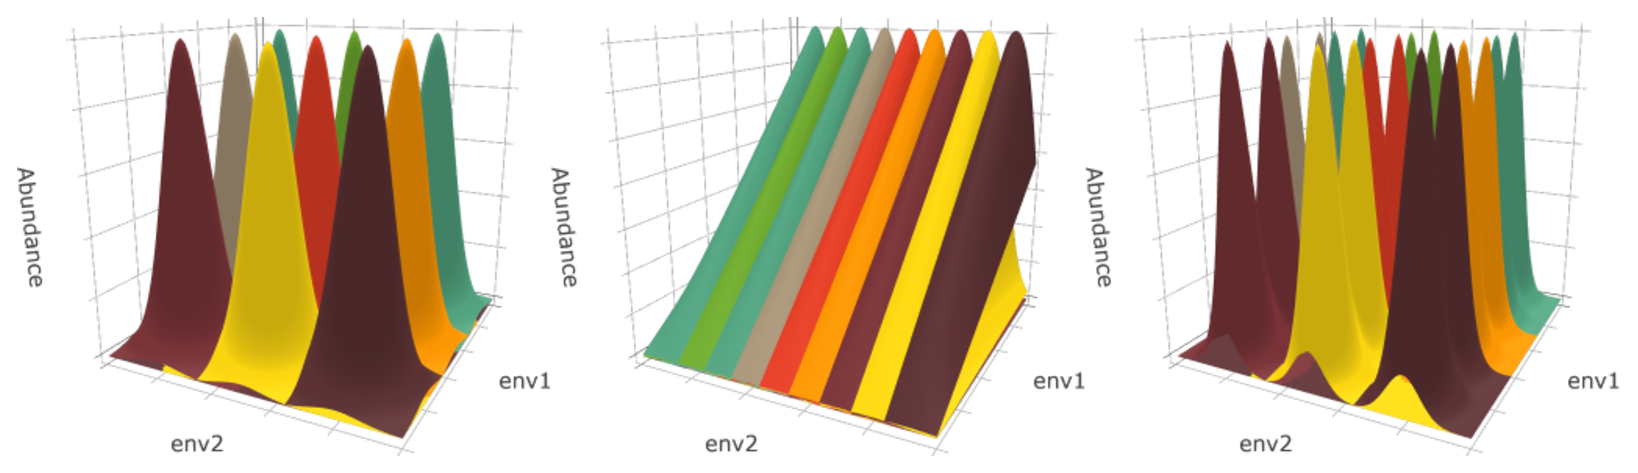
\includegraphics[width = 1\linewidth]{figure1_simulated_communities}   
			   	\caption{
			                Simulated abundance responses along two causal variables (\textit{env1} and \textit{env2}). 
                            Response combinations are: unimodal-unimodal (left), unimodal-linear (middle) and unimodal-bimodal (right). 
                			The vertical axis indicates abundance. 
                			The different colors represent different species.
                			All the examples show the unsampled abundance matrix
                			$\mathbf{Y_{Large}}$.
			            }
			    \label{fig:bivariateExample} 
			\end{center}
        \end{figure}
        
		%------------------------------%
		%&		Environmental Gradients				
		%------------------------------%        
        %
		We simulated abundances along two environmental gradients \textit{env1} and \textit{env2}, which henceforth will be referred to as causal variables to differentiate them from the noise variables.  
		%
        Both causal variables consist of the natural numbers from 1 to 100. 
        %
        Each possible combination of the two is a site, i.e. the total number of sites N = 10.000.
		%
		$\mathbf{Y_{Large}}$ holds the simulated abundances for all 10.000 sites.
	    %
	    This data set is larger than most ecological field data sets and fitting models to it would have required considerable computation time.
	    %
	    Therefore, we sampled from $\mathbf{Y_{Large}}$ with six different samples sizes (25, 100, 225, 400, 625, and 900) to obtain $\mathbf{Y_{Sample}}$.
        %
        Depending on the sample size $n$, a set number ($\sqrt{n}$) of sampling locations per causal variable were chosen. 
        %
        These locations always included the variable's minimum and maximum values (i.e. 1 and 100), between those, the locations were equidistantly distributed.
		%
		The abundances of all species at all combinations of sampling locations constitute $\mathbf{Y_{Sample}}$.
		%
		All species show the same response type towards each causal variable, but response types can differ between variables (Figure \ref{fig:bivariateExample}). 
	    %
		This setup allows for six communities each with a different combination of response types, including those with identical response types to both variables (Figure \ref{fig:flowchart_simulation}).  
		%
		The communities are labeled with their abbreviated response types, e.g. \textit{LB} for a community  in which species' abundances respond linearly to the first and bimodally to the second causal variable (Figure \ref{fig:bivariateExample}c). \\
		%------------------------------%
		%&		Responses				
		%------------------------------%
		Unimodal responses were simulated using the Gaussian response model \citep{GauchJr1972} expanded to multiple dimensions (Eqn. \ref{eq:GaussianResponseModel}).
		%
		\begin{equation} \label{eq:GaussianResponseModel}
					y_{s, n} = \prod_{m}^{M_{uni}} c_{s,m} \times exp\bigg(-\frac{(x_{m,n} - u_{s,m})^2}{2t^2_{s,m}}\bigg)		
		\end{equation}
		%	
    	where $u_{s,m}$ is the position of the optimum (i.e. the point with the highest abundance) of species $s$ along the environmental variable $m$, $t_{s, m}$ is the tolerance of species $s$ toward that variable and determines the width of the unimodal curve and $c_{s,m}$ is the maximal abundance of species $s$ on environmental variable $m$. 
		%
		$M_{uni}$ is the number of unimodal environmental variables. 
		%
		Linear responses were simulated by multiplying the environmental variables with a coefficient $\beta$ (Eqn. 2).
		%
		\begin{equation}
		 				y_{s,n} = \prod_{m}^{M_{lin}} x_{m,n} \times \beta_{s,m}
		\end{equation}
		%
		Bimodal responses were simulated by adding two unimodal models with different optima $u_{s,m}$.\\
		%
		This way we obtained $M = 2$ abundance values $y_{m,s,n}$ per species and site. 
		%
		To obtain a single abundance $y_{s,n}$ for each species at each site, we multiplied the abundances of each environmental variables.
		%
		By multiplying instead of adding the abundance values, we ensured that a species is absent from sites where its abundance drops to zero for one of the gradients, i.e. is outside of its niche. 

	%------------------------------%
	%&		Figure: Flowchart 	
	%------------------------------%
		
		\begin{figure}[ht]
			\centering
			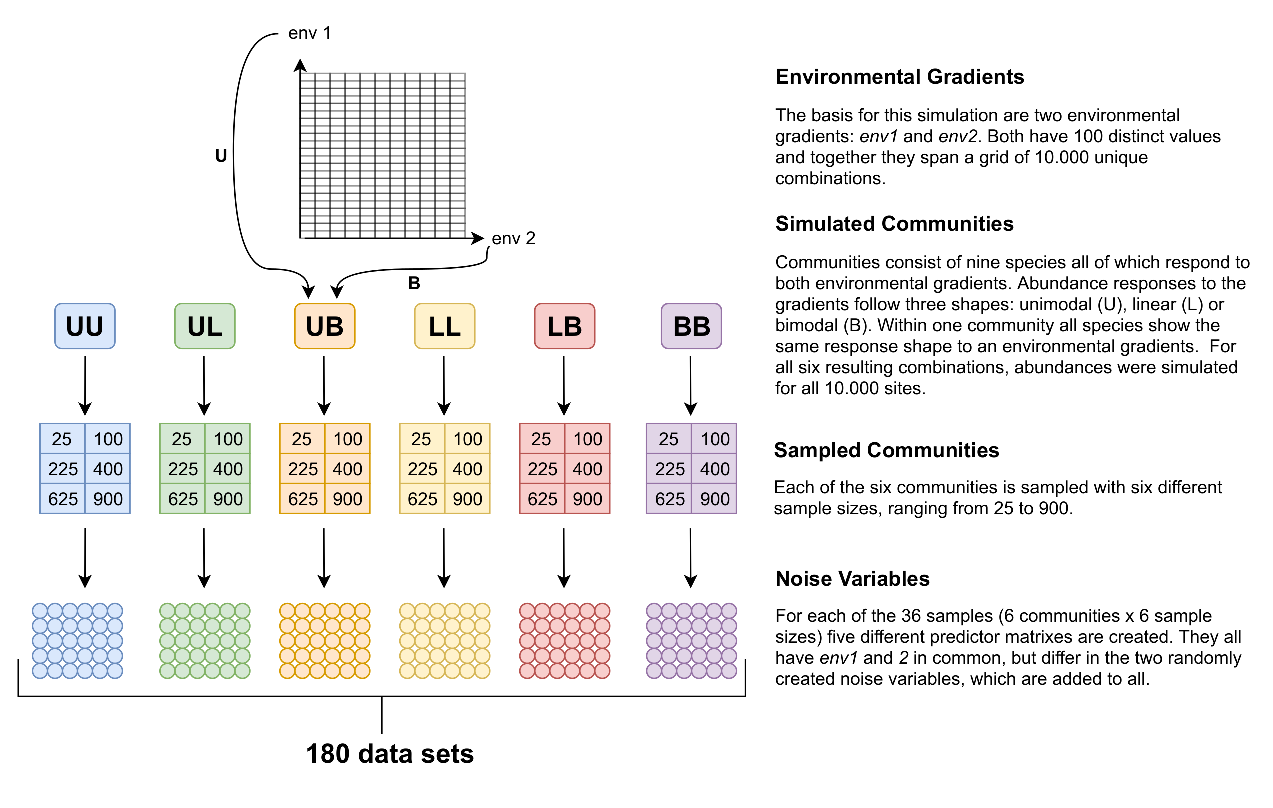
\includegraphics[width=1\linewidth]{manuscript/figure2_flowchart}
			\caption{
			        Flowchart of the community simulations. 
			        The environmental space is comprised out of two variables (\textit{env1} and \textit{env2}) and 10.000 unique sites.
			        At each site, the abundances of nine species are simulated. 
			        Abundance responses to environmental gradients display three shapes:
			        unimodal (U), linear (L) and bimodal (B). 
			         All nine species of one community show the same response shape (with varying parameters) to one gradient, but response shapes can differ between gradients. 
			         All six possible combinations of response shapes are sampled with six different sample sizes spanning from 25 to 900.
                    Before these data are analyzed two noise variables are added to $\mathbf{X}$ .
                    For each response shape - sample size combination, five different pairs of noise variables are appended to $\mathbf{X}$. 
			        }
			\label{fig:flowchart_simulation}
		\end{figure}
	
	%------------------------------%
	%&		Model MISC	
	%------------------------------%
	    
		%
		After the abundances were simulated, noise variables were appended to the model matrix $\mathbf{X}$.
		%
		They were simulated from a standard normal distribution, scaled to the same magnitude as the causal variables and restricted to be orthogonal to them and to each other.  
		%
	    We obtained five different versions of these noise variables by altering the random number generation seed,  giving us five different model matrices per sampled community $\mathbf{Y}_{Sampled}$.  
	    %
	    In total, we sampled six different communities six times each and have five model matrices per sample, resulting in 180 data sets per method of data analysis.\\
		%
        The simulated communities are a simplification of ecological field data. 
        %
        They consist of only nine species and are neither high dimensional nor do they exhibit intercorrelation.
        %
        However, they are not normally distributed and sparse, thereby featuring two of the common issues mentioned above. 
        %
        This relative simplicity eases interpretation of the results.
        %
        Finally, each model was run using five different seeds for random number generation which affects the noise variable. 
        %
        More details on the parameterization of the models are provided in Table SM 1.

    
    \subsection*{Overview of Methods}
        
        In the following, the methods of data analysis will be introduced briefly. 
        %
        Each section is concluded with details on how we applied the method in this study.  \\
        %
%     \subsubsection*{Multivariate Generalized Linear Models}
% 		A MvGLM consist of $S$ separately fitted univariate GLMs. 
% 		%
% 		The likelihood ratio test statistics of all univariate models (i.e. species) are added for each environmental variable to obtain the sum-of-likelihood-ratios statistics.  
% 		%
% 		For these statistics, \textit{p}-values related the null hypothesis that a given environmental variable has no effect on the mean community abundance can be calculated. 
% 		%
% 		We fit MvGLMs with Poisson, negative binomial and Gaussian residual distributions to each community and compared their Dunn-Smyth residual-plots \citep{dunn1996randomized} and Akaike's Information Criteria \citep[AIC, ][]{akaike1974new}.
% 		%
% 		The likelihood ratio test statistic was calculated for the best fitting model (least patterns in residuals and lowest AIC).
% 		%
% 	    To estimate \textit{p}-values, we used a residual permutation bootstrap with 1000 repetitions \citep{davidsonbootstrap}.
	
% 	%------------------------------%
% 	%&  CQO
% 	%------------------------------%
%         \subsubsection*{Constrained Quadratic Ordination}
% 	    Like the MvGLM, the CQO is related to the GLM. 
% 		%
% 		It is based on Vector Generalized Linear Models (VGLMs), which are a further generalization of GLMs.
% 		%
% 		All GLMs are special instances of VGLMs, just like linear regression is a special instance of a GLM.
% 		%
% 		They are not restricted to the exponential family, include multivariate response models, and can explicitly model other response parameters than the mean (e.g. the variance or higher order moments).
%         %
%         CQO builds on Reduced Rank-VGLMs, in which the $M$ original predictors are reduced to $R$ latent variables $\nu$. 
% 		%
% 		This entails the reduction of the hat matrix $\mathbf{H}$, which holds the regression coefficients $\beta$, to a rank $R$ matrix $\mathbf{H_R}$.
% 		%
% 		So unlike a MvGLM, CQO reduces the data's dimensionality and in contrast to most ordination techniques (including dbRDA and CCA), the researcher specifies the number of latent variables (i.e. dimensions)  \textit{a priori}.
% 		%
% 		$\mathbf{H_R}$ is decomposed into two matrices $\mathbf{H_R}^T = \mathbf{A}\ \mathbf{C}^T$, where $\mathbf{H_R}^T$ denotes the transpose of $\mathbf{H_R}$.  
% 		%
% 		The latent variables $\mathbf{\nu}$ are the linear combinations of the constrained coefficients $\mathbf{C}^T$ and the sites-by-predictor matrix $\mathbf{X}$.
% 		%
% 		This means that the higher the constrained coefficient of a given predictor is, the more influence it has on the corresponding latent variable.   
% 		%
% 		$\mathbf{A}$ holds the regression coefficient of the latent variables.
%         %
% 		CQO extends this model by adding a quadratic term (cf. Eqn. \ref{eq:CQO1}). 
	
% 		\begin{equation}\label{eq:CQO1} 
% 		\eta_s = \beta_{(s)1} + \beta_{(s)2} \nu + \beta_{(s)3} \nu^2	
% 		\end{equation} 
		
% 		$\beta_1$ is the intercept term and $\eta$ is the linear predictor. 
%         It assumes symmetric and unimodal responses to the latent variables.
% 		 % 
% 		CQOs were run with Poisson residual distribution and the canonical log-link function.
% 		%
% 		The four explanatory variables were scaled and centered before fitting the models.
% 		%
% 		The effective nonlinear degrees of freedom were set to 1.5 as suggested by \citet{yee2015vector}.
% 		%
% 		Each model was run fifty times and the deviances of each run were compared. 
% 		%
% 		If the lowest deviances are too far apart, the solution might be local and the model should be refitted.  
% 		%
% 		Here, we fit the model again, until the difference between the lowest and the fifth lowest deviance no longer exceeds 3. 
% 		% 
% 		% General Info - absolute values 
%         In its current implementation in the VGAM R-package \citep{VGAM19}, CQO does not provide \textit{p}-values \cite[but see][]{yee2010vglms}. 
%         %
%         To compare its results with the other methods, we calculated pseudo-\textit{p}-values for the CQO (details of the procedures can be found in the 
%         %section 2 of the Supplementary Materials).
%         Appendix).
%         %
%         Shortly, to determine the pseudo \textit{p}-value of environmental variable \textit{m}, we permuted the variable 100 times and fit a CQO to each permuted data set. 
%         %
%         For every model, the absolute values of the constraint coefficient across both latent variables were added for environmental variable \textit{m}, to obtain the test statistic $\sum C_{\nu_{X_{m}}}$. 
%         %
%         The proportion of test statistics of permuted data sets, that were larger than that of the unpermuted data set, is the pseudo-\textit{p}-value. 
%         %
% 	    All models were fit with rank 1 and 2.
% 		%
% 		The optimal number of ranks was found to be 2 for all models, determined by the AIC as proposed by \citet{yee2003reduced}.\\

% 	%------------------------------%
% 	%&  CCA
% 	%------------------------------%
% 	\subsubsection*{Canonical Correspondence Analysis}
% 	 CCA is the heuristic solution to Restricted Gaussian Regression \citep{Zuur2007}. 
% 	 %
% 	 In the latter, one tries to estimate the parameters \textit{u}, \textit{t}, and \textit{c} of a Gaussian response model (see Eqn. \ref{eq:GaussianResponseModel}), but instead of the measured environmental variables, their linear combinations are used as $x$. 
% 	 %
% 	 Though it is possible to estimate the parameters with iteratively reweighted least squares in a GLM, this was to computationally intensive at the time the method was proposed by  \citet{GauchJr1972}.
% 	 %
% 	 Instead, \citep{TerBraak1986} proposed to approximate the results by CCA, which is valid as long as: all species have equal tolerances $t$ and maximal abundances $c$, their responses are unimodal and symmetrically bell-shaped and their optima $c$ are spread uniformly in the ordination space. 
% 	 These assumptions are collectively known as the \textit{species packing model}.
% 	 %
% 	 \citet{Palmer1993}, \citet{Johnson1999} and \citet{Zuur1999} confirmed the validity of the approximation and its robustness towards violations against the species packing model in simulation studies.
% 	 %
% 	 Today, CCA is one of the most widely used and cited multivariate statistical methods in ecology \citep{Braak2014}.\\
% 		%
% 		An iterative algorithm is used to obtain estimates. 
% 		%
% 		First, arbitrary values are assigned to the site scores (positions of sites in latent variable space, $\mathbf{Z}$). 
% 		%
% 		These are used to calculate the species optima $u$ (henceforth species scores) as in Eqn. \ref{eq:CCA_species_scores}.
% 		%
% 		\begin{equation}\label{eq:CCA_species_scores}
% 		\mathbf{u} = \mathbf{D}_c \mathbf{Y}^t \mathbf {Z}
% 		\end{equation}
% 		%
% 		Where $\mathbf{u} = (u_1\ ...\ u_S)^t$, $\mathbf{D}_c$ is a diagonal matrix with the abundance of species $s$ across all sites as its $s,s$-th element and $\mathbf{Y}^t$ denotes the transpose of $\mathbf{Y}$.
% 		%
% 		The species scores are in turn used to calculate the site scores as their weighted average $\mathbf{Z}_{wa}$ (Eqn. \ref{eq:CCA_site_scores}) 
% 		%
% 		\begin{equation} \label{eq:CCA_site_scores}
% 			\mathbf{Z}_{wa} = \mathbf{D}_r^{-1} \mathbf{Y} \mathbf {u}
% 		\end{equation}
% 		%
% 		where $\mathbf{D}_r$ is a diagonal matrix with the abundance of all species at site $n$ as its $n,n$-th element and $\mathbf{D}_r^{-1}$ denotes the inverse of $\mathbf{D}_r$. 
% 		%
% 		$\mathbf{Z}_{wa}$ is regressed against $\mathbf{X}$ to obtain the weighted regression coefficient $\alpha$. 
% 		%
% 		\begin{equation}\label{CCA_canocical_weights}
% 		\alpha = (\mathbf{X}^t \mathbf{D}_r \mathbf{X})^{-1} \mathbf{X}^t \mathbf{D}_r \mathbf{Z}_{wa}
% 		\end{equation}
% 		%
% 		Lastly, $\mathbf{Z}$ is calculated as the product of $\mathbf{X}$ and $\mathbf{\alpha}$. 
% 		%
% 		This procedure is repeated until convergence. \\
% 	    %
% 		The distance between sites (scaling 1) or species (scaling 2) in a CCA approximates their two-dimensional $\chi^{2}$-distance, i.e. the Euclidean distance between the expected abundances under the null hypothesis, that abundances do not change along environmental variables, and the actual data.
% 		%
% 		Explanatory variables were scaled and centered. 
% 		%
% 		Hypothesis tests for environmental variables can be conducted using a pseudo-$F$ statistic with permuted residuals  \citep{Legendre2011} and the null hypotheses that the effect of the variable on the response is equal to zero after accounting for the effect of all other variables. 
% 	    %
% 	    Hypothesis tests were conducted with 999 permutations.\\
	
% 	%------------------------------%
% 	%& dbRDA
% 	%------------------------------%
% 	\subsubsection*{distance-based Redundancy Analysis}
% 	    dbRDA is a variation of the commonly used Redundancy Analysis, proposed by \citet{Legendre1999}.
% 	    %
%         It is not based on one specific distance measure but instead can adopt any chosen measure.
%         %
% 		It is the constrained form of Principal Coordinates Analysis (PCoA) \citep{Legendre1999}, which will be shortly addressed here.
% 		%
% 		In PCoA, $\mathbf{Y}$ is transformed into a centered distance matrix $\Delta$.
% 		%
% 		The columns of the matrix $\mathbf{PC}$ are the eigenvectors of $\Delta$ scaled to a length that is equal to the square root of their eigenvalues \citep{gower1966some}.
% 		%
% 		Each row of PC gives the eponymous \textit{Principal Coordinates} of one observation.
% 		% 
% 		In a dbRDA, this matrix $\mathbf{PC}$ is linearly related to the explanatory variables by an RDA.
% 		%
% 		The dbRDA preserves the distance metric of $\Delta$, which can be metric, semi- or non-metric.
% 		%
% 		dbRDA was highlighted by \citet{Szocs2015}, because the possibility to use asymmetrical distance metrics makes them appealing for sparse data sets. 
% 		%  	
% 	    We used the Bray-Curtis distance, which is the reciprocal of the Steinhaus coefficient  \citep{motyka1947zadaniach}, to calculate $\Delta$.
% 	    %
% 		Negative eigenvalues were corrected with Lingoes correction \citep{lingoes1971some}.
% 		%
% 		As in CQO and CCA, environmental variables were scaled and centered. 
% 		%
% 		The significance tests for explanatory variables are calculated using a pseudo-F-Statistic in the same manner as for the CCA.\\
		
% 	\subsection*{Comparison of Methods}
%         % How did I evaluate the methods look at results
%         The benefit of using simulated rather than field data are twofold:
%         %
%         i) there is a clear dichotomy between causal and noise variables and 
%         ii) we know which variable belongs to which group. 
%         %
%         This enables us to compare the methods in terms of their classification error rates.
%         %
%         To this end, we calculated false positive (FPR) and false negative rates (FNR) for each method.
%         %
%         % \begin{align}
%         %   FPR &= FP /(TN + FP) \\        
%         %   FNR &=  FN / (TP + FN)
%         % \end{align}
%         where FP is a False Positive, TN a True Negative, FN a False Negative, and TP a True Positive. 
%         %
%         A false positive occurs when a noise variable is classified as causal, whereas a false negative when a causal variable is classified as non-causal. 
%         %
%         True positives and negatives are instances where the variable is labeled correctly. 
%         %
%         An FPR of 0.5 for example would indicate, that half of all noise variables were classified as causal. 
%         %
%         Variables with a \textit{p}-value lower than the significance level($\alpha$) were classified as causal whereas all variables with $p > \alpha $  were classified as noise.
%         %
%         To alleviate the problematic dichotomy of statistical significance \citep{Greenland2016}, we use five different significance levels $\alpha$ (0.01, 0.03, 0.05, 0.07 and 0.1).
% 		%
% 		This allows us to evaluate trends in classification strength over different thresholds. 
        

% 	\subsection*{Software}
% 		All simulations and analyses were done in R 3.4.4 \citep{RCT2018}.
% 		%
% 		MvGLM were conducted with mvabund 3.13.1. \citep{Wang2019}, dbRDA and CCA with vegan 2.5-2 \citep{Oksanen2018} and CQO with VGAM 1.0-5 \citep{VGAM19}. 
% 		%
% 		%
% 		All calculations were conducted on an Ubuntu 18.04 machine with 64-bit, 8 GB RAM and 1.6 GHz.\\
% 		%
% 		All datasets and R scripts generated during and/or analysed during the current study are available from the corresponding author on reasonable request.

% \section{Results}
% 		%------------------------------%
% 		%& 		References 				
% 		%------------------------------%  
	
% 		We report the means and standard deviations of \textit{p}-values of MvGLM, CQO, CCA, and dbRDA for all explanatory variables (Table \ref{table:results1::mean-p}), p-values for different response shapes and sample sizes are given in the Tables S 2 - 5.
		
% 		%------------------------------%
% 		%& Table: p-values + standard deviations
% 		%------------------------------% 

%         \begin{table*}[ht]
%             \centering
%         	\caption{
%         	    Mean \textit{p}-values $\pm$ standard deviations of the causal (env1 and env2) and noise variables from multivariate Generalized Linear Models (MvGLM), Constrained Quadratic Ordination (CQO), Canonical Correspondence Analysis (CCA), and distance-based Redundancy Analysis (dbRDA) for all models. 
%         	    }
%             \begin{tabular}{@{}
%             >{\columncolor{white}[0pt][\tabcolsep]}
%             cccc
%             >{\columncolor{white}[\tabcolsep][0pt]} c
%             @{}}
%                 \rowcolor{lightgray}
%                 & \textbf{MvGLM} & \textbf{CQO}      &  \textbf{CCA}     & \textbf{dbRDA} \\
%                 \toprule
%                 \textit{env1}  & $0.006 \pm 0.0275$   & $0.067 \pm 0.127$ & $0.264 \pm 0.433$ & $0.002 \pm 0.007$ \\
%                 \textit{env2}  & $0.009 \pm 0.0311$   & $0.090 \pm 0.190$ & $0.264 \pm 0.433$ & $0.003 \pm 0.011$ \\
%                 Noise          & $0.650 \pm 0.280$    & $0.680 \pm 0.268$ & $0.399 \pm 0.348$ & $0.523 \pm 0.256$ \\
%                 \bottomrule  
%             \end{tabular}
%             \label{table:results1::mean-p}	
%         \end{table*}


% 	%------------------------------%
% 	%& 		GLMmv 					
% 	%------------------------------%
% 		%------------------------------%
% 		%& 			In General 			
% 		%------------------------------%
%         In most MvGLMs, negative binomial residual distribution achieved the lowest AIC and the best fit to model assumptions. 
% 		%  
% 		The plot of Dunn-Smyth residuals against the linear predictor of \textit{LL} (Figure S 1) showed arched patterns, which could indicate that the residuals were not independent of the explanatory variables. 
%         %
%         Nevertheless, We used a negative binomial residual distribution because visual inspection of the QQ-Plots suggested that it resulted in a better fit than Poisson or Gaussian distributions. 

% 		%------------------------------%
% 		%& 	 p-values 	
% 		%------------------------------% 
% 		MvGLMs' \textit{p}-values for both causal variables and all response type combinations were low (Table  \ref{table:results1::mean-p}).
% 		%
%         The \textit{p}-values of the linear variable in \textit{LB} and \textit{UL} and of the bimodal variable in \textit{UB} were higher at the smallest sample size than at higher ones (Table S 2).  
% 		%
% 		Otherwise, the samples size had no effect on the \textit{p}-values of the causal variables, which often were minimal (1 divided by the number of permutations + 1) at small sample sizes.
% 		%
% 		The \textit{p}-values for noise variables were higher and varied strongly (Figure \ref{fig:result1::p-valueComparison}).
% 		%
% 		They only fell below the nominal significance level of 0.05 in three models. 
% 		%
% 		All three models had the response combination \textit{LL} and the low \textit{p}-values occurred at the sample sizes 225, 625, and 900 (Table S 2).
% 		%
% 		%------------------------------%
% 		%& 	 FPR/ FNR  	
% 		%------------------------------%
% 		%
% 		The FPR was the lowest of all methods (0.008 at $\alpha = 0.05$) and always well below the respective significance level (Figure 3). 
% 		%
% 		Overall, FPRs and FNRs of MvGLMs were very low (Figure \ref{fig:FPNR}).
% 		%
%         Interestingly the \textit{p}-values of noise variables did not show a monotonic positive relationship with samples size, as we expected. 
%         %
%         Rather the response seemed unimodal in \textit{UU}, \textit{LL}, and \textit{BB}, slightly negative in \textit{LB} and \textit{UL} and positive for \textit{UB} (Table S 2). \\ 
        
%         \begin{figure}[h]
%             \centering
%             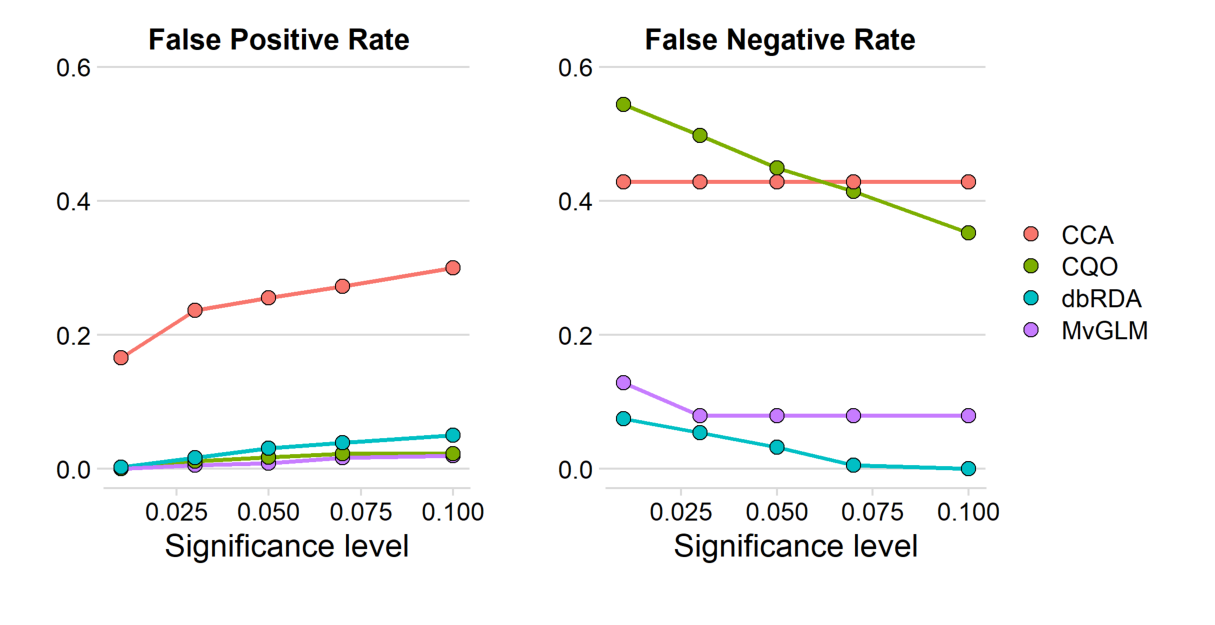
\includegraphics[scale = 0.7]{FPNR}
%             \caption{False Positive Rate and False Negative Rate of the four statistical methods Canonical Correspondence Analysis (CCA), Constrained Quadratic Ordination (CQO), distance-based Redundancy Analysis (db-RDA), and multivariate Generalized Linear Model (MvGLM). }
%             \label{fig:FPNR}
%         \end{figure}{}
                    
%     %------------------------------%
% 	%& 	CQO			
% 	%------------------------------% 
	
% 	CQOs performance strongly depended on the response shape (Figure \ref{fig:result1::p-valueComparison}). 
%     %
%     It failed to converge for \textit{UB} with sample size 25 and performed best for \textit{UU} and \textit{BB}; both had a FNR of 0 FPRs below the average (0 and 0.06 respectively).
%     %
%     \textit{UB} performed slightly worse than \textit{UU} and \textit{BB} with an FNR of 0.1 and an FPR of 0.02.
% 	%
% 	As was expected, CQO often assigned high \textit{p}-values to linear causal variables (Figure \ref{fig:result1::p-valueComparison}). 
% 	%
% 	The mean \textit{p}-value of linear variables was 0.15 and their FNR was 0.53. 
% 	%
% 	Both unimodal and bimodal causal variables received higher \textit{p}-values when the other causal variable was linear (Table S 3).
% 	%
% 	The mean \textit{p}-value of unimodal variables excluding those from \textit{UL} is $0.006\pm0.022$ compared to $0.036\pm0.084$ for the unimodal variable in \textit{UL}.
% 	%
% 	Similarly, the mean \textit{p}-value of bimodal variables except for those form \textit{LB} is $0.004\pm0.015$ and for the bimodal variable in \textit{LB} it is $0.042\pm0.083$.
% 	%
%     This mixed performance leads to relatively high mean \textit{p}-values for the causal variables (Table \ref{table:results1::mean-p}) and accordingly high FNR and FPR (Figure \ref{fig:FPNR}).\\
    
%     % --------------------------------------------------------
%     %& False negative positive figure 
    
%     \begin{figure}
%         \centering
%         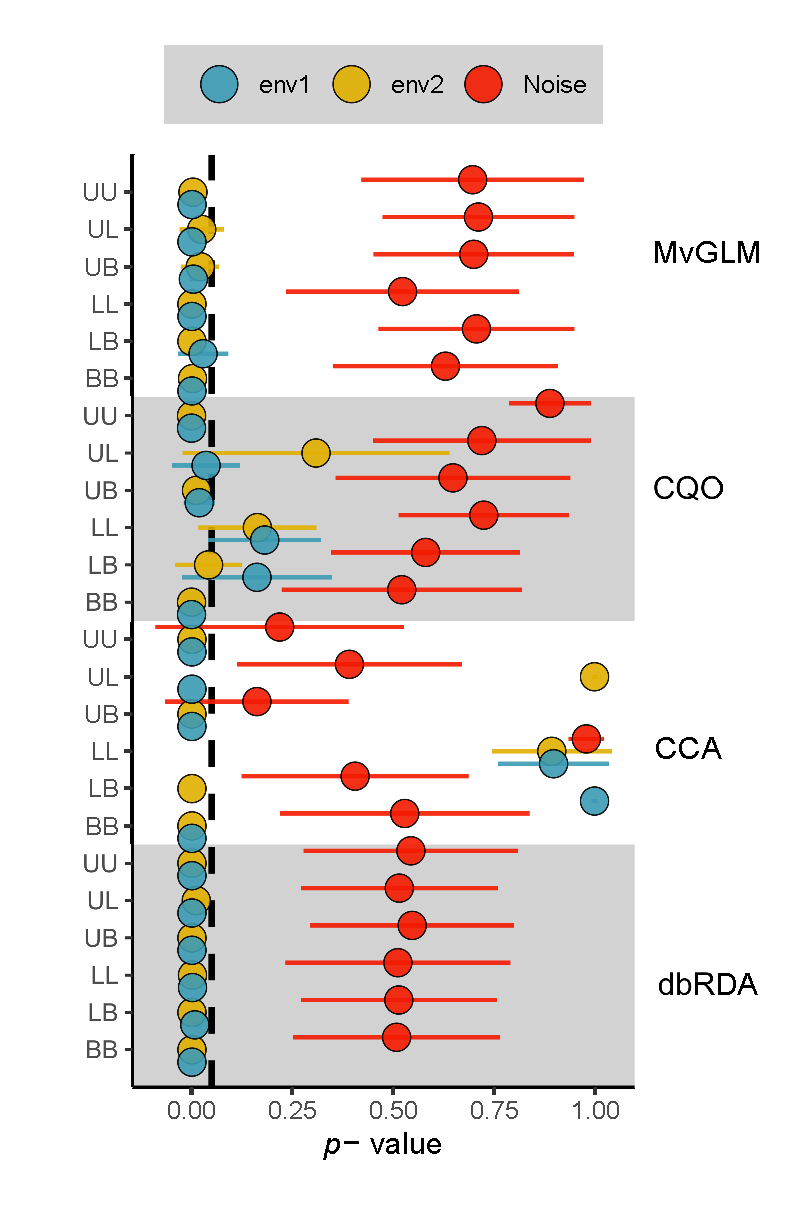
\includegraphics[scale = 0.7]{190912_error_bar}
%         \caption{Mean \textit{p}-values of response combinations (indicated by first letter of response types: unimodal (U), linear (L), bimodal (B)) for multivariate Generalized Linear Models (MvGLM), Constrained Quadratic Ordination (CQO), Canonical Correspondence Analysis (CCA), and distance-based Redundancy Analysis (dbRDA). Blue points are \textit{env1}, yellow points \textit{env2} and red points are noise variables. Bars show one standard deviation. The vertical, dashed line indicates a \textit{p}-value of 0.05.}
%         \label{fig:result1::p-valueComparison}
%     \end{figure}
%     % --------------------------------------------------------
    
    
%     %------------------------------%
% 	%& 			CCA					
% 	%------------------------------% 

% 		%------------------------------%
% 		%& 			Variables			
% 		%------------------------------% 

% 		CCA has the highest mean \textit{p}-values for causal variables and the lowest for noise ones. 
% 		%
% 		Accordingly, the FPR was the highest of all methods (Figure \ref{fig:FPNR}.
% 		%
% 		Irrespective of significance level, it is more than one order of magnitude higher than for all other methods.
% 		%
% 		These problems are due to two factors: i) high \textit{p}-values for causal linear variables and ii) low \textit{p}-values for noise variables. 
% 		%
% 		The mean \textit{p}-value for causal linear variables is $0.963\pm0.094$. 
% 		%
%         Additionally, CCAs of \textit{LL} with sample sizes 400 to 900 produced constrained inertias (explained variance) of 0 and were therefore excluded from significance testing. 
% 		%
% 		Noise variable \textit{p}-values were especially low in \textit{UU} and \textit{UB} (Figure \ref{fig:result1::p-valueComparison}), which is interesting since these data sets matched closest with the assumed \textit{species packing model}.  
% 		%
% 		In \textit{BB} they were markedly higher (Table S 4). 
% 		%
%         The impact of different sample sizes was negligible in all response combinations (Table S 4).   

% 	%------------------------------%
% 	%& 	db-RDA 	
% 	%------------------------------%

% 		The dbRDA assigned low \textit{p}-values to most causal variables (Figure \ref{fig:result1::p-valueComparison}).
% 		%
% 		The only \textit{p}-values of causal variables above the nominal significance level of 0.05 were those of linear variables at a sample size of 25 (Table S 5).
% 		%
% 		However, they were below 0.1, so that the dbRDA had an FNR of 0 at $\alpha = 0.1$.  
% 		%
% 		Indeed, the FNR was the lowest of all methods (Figure \ref{fig:FPNR}).
% 		%
%         The \textit{p}-values were relatively similar for all sample sizes (Table S 5). 
% 		%
%         The FPR of dbRDA was relatively high, with 0.031 at $\alpha = 0.05$.  
%         %
%         The FNR was the lowest of all methods. \\
%         %
%         Both algorithm-based methods were considerably faster than the model-based ones (Figure S 2).

% % !TeX spellcheck = en_US
% \section{Discussion}
% %------------------------------%
% %& 		Repeat what I did		
% %------------------------------%
% 	We analyzed 180 simulated abundance data sets, that differed in response types and sample sizes with four different statistical methods, to assess the methods performance when used to differentiate between causal and noise variables. 
	
% %------------------------------%
% %& 	one sentence conclusions	
% %------------------------------%

%     MvGLM and dbRDA performed best showing low FPRs and FNRs for all response combinations and sample sizes. 
% 	%
%     CQO assigned high \textit{p}-values to noise variables resulting in FPRs lower than those of dbRDA but higher than MvGLM's. 
%     %
%     However, it had the highest FNR for the lower three significance levels, resulting largely from the high \textit{p}-values of linear variables. 
% 	%
%     CCA also assigned high \textit{p}-values to linear variables and additionally assigned low \textit{p}-values to noise variables. 
%     %
%     The method performed worst in this evaluation, showing the highest FPR at all significance levels and the highest FNR at the two highest significance levels. \\
	
% %------------------------------%
% %& 			GLMmv				
% %------------------------------%
    
%     MvGLMs had the lowest FPR of all methods. 
%     %
%     The three noise variable \textit{p}-values that fell below 0.05 all occurred in \textit{LL} models, which violated the assumption of random residuals and thus would likely be identified as unreliable models.
% 	%
% 	The FNR was also low and resulted only through communities with the smallest sample size.
% 	%
% 	A drawback of MvGLMs is the long run time due to resampling \citep{Wang2012}.
% 	%
% 	The resampling is necessary because it ensures that inferences are valid, even if species are intercorrelated. 
% 	%
% 	Resampling observations across independent sites (i.e. rows) accounts for their possible correlation \citep{anderson2001new}. 
%     %
% 	Models that explicitly consider correlation structure avoid resampling and can reduce computation time.
% 	%
% 	Such models have been proposed, e.g. by \citet{Jamil2012} who used the site effect of a Generalized Linear Mixed Model to induce equal correlation between all species pairs.
%     %
%     A clear drawback of this method is, however, that equal correlation between all species is as (im)plausible as no correlation. 
%     %
%     Structuring the residual covariance matrix is important as the number of parameters that need to be estimated rises quickly (e.g. 55 in the covariance matrix for 10 species).
%     %
%     MvGLMs can use an unstructured correlation matrix, but this is only advisable for data sets with many more sites than species and is computationally expensive. 
%     %
%     Another option is shrinking the correlation matrix towards identity using ridge regularization \citep{warton2008penalized, Warton2011a}.
% 	%
% 	Both alternatives use Generalized Estimation Equations (GEE) with the sandwich-type-estimator of \citet{Warton2011a}.
% 	%
% 	As GEEs do not provide likelihoods, other test statistics than the Likelihood ratio have to be used. 
% 	%
% 	Current options are the score and the Wald statistic.
% 	%
% 	However, these methods also require resampling, as asymptotic marginal distributions of regression parameters for GEEs are not specified for data sets with more species than sites.
% 	%
%     Testing these methods on data sets with known correlation structures could highlight stronger performance differences, as the other methods lack adjustments to these properties.
%     %
% 	MvGLMs are the only method considered here that does not reduce the dimensions of the data.
% 	%
% 	Visualizing the multidimensional data is difficult as no easy-to-use and interpret method for MvGLMs is available. \\

% %------------------------------%
% %& 		dbRDA		
% %------------------------------%
%     dbRDA was least influenced by different response types and sample sizes. 
%     %
%     These properties, together with the low FPR and FNR and the modest computation time make it an excellent method for cultivate analysis in ecology.
% 	%
% 	However, the FPR was higher than that of both model-based methods.
% 	%
% 	Small \textit{p}-values were scarce for noise variables but occurred at all samples sizes and response types. 
% 	%  
% 	dbRDA's good performance is in concert with other simulation studies \cite[e.g.][]{Roberts2009}.
% 	%
% 	These results are only valid for the Bray-Curtis distance metric, which was used here.
% 	%  
% 	Other measures would likely produce different results, 
% 	therefore the selection of an appropriate metric is a crucial step in any dbRDA analysis.
% 	%  
% 	Having to choose a single metric can be avoided by using consensus RDA \citep{Blanchet2014}.
% 	% 
% 	In this method, multiple dbRDAs are run, only differing in their distance metric. 
% 	%
% 	Site scores on statistically significant axes are combined into one matrix, which acts as a response matrix in a new RDA. 
% 	%
% 	This method extracts the information that is common to all individual dbRDAs.
% 	%
% 	Simulation studies comparing properties of consensus RDA with those of individual dbRDA and other methods, algorithm- or model-based, are lacking.
% 	% 
% 	Another avenue for the future development of distance-based algorithms, in general, would be novel distance metrics, but their development is pending (M. J.Anderson, pers. comm.).\\

% %------------------------------%
% %& 				CCA				
% %------------------------------%

% 	The CCA performed worst of the methods tested and assigned high \textit{p}-values to all linear variables.
% 	%
% 	As CCA assumes unimodal gradients, which are more frequent than linear ones in nature \citep{Oksanen2002}, this was expected.  
% 	%
% 	This study confirmed, that CCA should be avoided if exploratory analyses indicate linear relationships, which can occur if the sampled range of a gradient is short relative to the species' tolerance. 
% 	%
% 	Noise \textit{p}-values were lower than in other methods.
% 	% 
% 	Most of the low \textit{p}-values for noise variables occurred in communities with uni- or bimodal responses. 
% 	%
% 	This is surprising, given that \textit{UU} fits the expectations of the species packing model perfectly and bimodal models deviate only slightly.
% 	%
% 	Newer approaches to CCA that can correct for zero inflation \citep{Zhang2012} or non-linear relationships between predictor and response variable \citep{Makarenkov2002} are available but not widely used. 
% 	%
% 	Indeed, all of the methods we tested here can include quadratic terms which would most likely have resulted in better fitting models for unimodal and bimodal predictors. 
% 	%
% 	Their application is uncommon in CCA and RDA and could be the scope of a future studies.

% %------------------------------%
% %& 			CQO					
% %------------------------------%

% 	Similar to the CCA, CQO assigned high \textit{p}-values to linear variables. 
% 	%
%     It also assumes unimodal responses and the non-detection of causal linear gradients was expected. 
%     %
%     The \textit{p}-values for linear variables of CQO were markedly lower than in the CCA, however, the \textit{p-value} of the second variable in these models tends to increase. 
%     %
%     Overall, this resulted in a high FNR.
% 	%
% 	The FPR however, was lower than for both algorithm-based methods but slightly higher than for MvGLM. 
% 	%
% 	These results reflect the performance of CQO when combined with our approach to compute \textit{p}-values, which to our knowledge, is novel. 
% 	%
% CQO has only rarely been used in ecological studies and mostly within fisheries research (e.g. \citet{Vilizzi2012}, \citet{Top2016} and \citet{Carosi2017}). 
% 	% 
% 	\citet{TerBraak2015} suggest that this is due to limitations on the number of species that can be included, a steep learning curve and numerical instability. 
% 	%
% 	This study confirmed that in its current state the method has issues with linear response types but can handle alteration of the symmetrical unimodal bell-shape. \\

% % ---------------------------------------- %
% %&		Andere Vergleichende Studien		
% % ---------------------------------------- %
 
%  	Our study is the first to directly compare the methods. 
%  	%
%  \citet{Warton2012} compared MvGLMs to CCA and RDA (not dbRDA).
%  	%
%  	They showed that only MvGLMs successfully differentiate between the location effect (difference in means) and dispersion effect (difference in variance). 
%  	%
%  	Comparative studies of multivariate methods, in general, are common. 
%  	%
%  	Especially ordination techniques like CCA and RDA were subject to extensive testing in the 1970s and 1980s \cite[e.g.][]{GauchJr.1972, GauchJr1977, Kenkel1986}. 
%  	%
%  	To our knowledge, \citet{Roberts2008} and \citet{Roberts2009} are the only studies that systematically compared dbRDA to other methods. 
%  	%
%  	Both compared dbRDA, CCA and Multidimensional Fuzzy Set Ordinations. 
%  	%
%  	\citet{Roberts2008} used simulated data sets to this end, whereas \citet{Roberts2009} used four different field data sets. 
%  	%
%  	Both studies concluded that dbRDA outperforms CCA, as it does in this study.
%  	%
%  	CQO is occasionally tested in comparisons of individual and community level species distribution models (e.g. \citet{Baselga2009} and \citet{Maguire2016}),
%  	where they are an instance of the latter.
%  	%
%  	Generally, they exhibited a similar performance as classical models (e.g. GLMs or Regression Trees). \\

% %------------------------------%
% %& 		Simulated Data			
% %------------------------------% 
%     The realism of the simulated communities could be improved by using more complex response patterns like beta-functions \citep{austin1994determining}, which add asymmetries to bell-shaped curves.
% 	%
% 	However, in a study of \citet{Oksanen2002} only about 20\% of the responses were strongly skewed, whereas symmetric and bell-shaped responses were most common. 
% 	%
% 	Alternatively, asymmetry could be introduced through random terms added to abundances, environmental variables, or both. \cite[e.g.][]{McCune1997}
% 	%
% 	When correlated random terms are added to both, this would engender endogeneity (a non-zero covariance between the residuals and one or more explanatory variables). 
% 	%
% 	Simulations with induced endogeneity would be interesting as this phenomenon is underappreciated by ecologists \citep{armsworth2009contrasting, fox2015ecological}.
% 	%
% 	Observation and measurement are sources of errors in field data sets, and both can be represented in a model via binomial functions as in N-mixture models \citep{royle2004n}.
% 	%
%     This would be interesting to examine the effects of regression dilution \citep{frost2000correcting, McInerny2011}.
 
% %------------------------------------------------%
% %& Andere Vielversprechende Model-based approaches
% %------------------------------------------------%

% 	Our study shows that model-based multivariate inference can outperform more frequently used algorithm-based methods. 
% 	%
% 	The answer to our eponymous question is thus: Not categorically - decisions should be made on a case-by-case basis.
% 	%
% 	As model-based methods are still at an early stage, new developments and increases in computation speed can be expected.   
% 	%
% 	An especially active area are models using joint probability distributions \cite[e.g.][]{Clark2014, Pollock2014} that estimate the joint distribution of all species conditional on the environmental variables instead of only using the marginal distribution of every species' abundance. 
% 	%
% 	A common interest of many joint models is to infer biotic interactions from the residuals of the species-environment interaction, 
% 	as these two sets of predictors (biotic and abiotic) were shown to have little redundancy \citep{Meier2010}.
% 	%
% 	Some of the models also anticipate the growing challenges of Big Data for ecology \citep{Hampton2013}.
% 	%
% 	Generalized Linear Latent Variable Models, for example, include latent variables instead of random effects to capture residual correlation, which considerably reduces the size of the variance -- covariance matrix \citep{Warton2015,Niku2017}.  
% 	%
% 	In Hierarchical Modeling of Species Communities \citep{Ovaskainen2017} this approach is coupled with a fourth corner model \cite[including species traits, ][]{legendre1997relating} and phylogenetic relationships to create a flexible and comprehensive framework for community data analysis.
% 	%
% 	In a similar vein, Generalized Joint Attribute Models allow for different kinds of data (e.g. continuous, discrete counts, ordinal counts, and occurrence) to be included in the same response variable and have outperformed Poisson GLM on discrete count data and a Bernoulli GLM on binary host status data in a recent simulation study \citep{Clark2017}. 
% 	%
% 	Lastly, \citet{anderson2019pathway} recently highlighted a combination of the model- and algorithm-based approaches.
%     %
%     They proposed a copula model of ecological count data \cite[see][for an introduction to copula models]{hofert2018elements}, which consists of i) fitting a copula model to the data, ii) simulating new count data with this copula and iii) visualizing the centroids of the actual data and of the simulated data sets in a PCoA.
%     %
%     In light of the good performance of dbRDA in our study, this proposal, to join features from both approaches, should be further pursued. 
%     %
% 	It is now essential that ways to infer ecological processes from the modeled patterns develop at a similar pace as these models, to avoid confusing statistical artifacts with genuine biological signals \citep{dormann2018biotic}.
% 	%
% 	If this succeeds, a move from algorithm-based towards model-based methods might entail one from the current implicit Gleassonian towards a modern form of Clementsian perspective \citep{Eliot2011}; from asking how do individual species change along environmental gradients towards asking how do communities change as a whole.   
	
% \section*{Acknowledgements}
% The authors wish to thank Andreas Scharmüller, Stefan Kunz, Sebastian Scheu, Verena Schreiber, and Lucas Streib whose valuable comments  improved the quality of the final document. The publication was funded by the Open Access Fund of the University of Koblenz-Landau.
% \section*{Author Contributions}
% JFJ and RBS conceived the experiment. JFJ conducted the simulation and the analyses. JFJ and RBS wrote the manuscript.
% \section*{Data accessibility}
% All data as well as R scripts are available in the associated Github repository (https://github.com/JonJup/Should-ecologists-prefer-model--over-algorithm-based-multivariate-methods). 
% %%% -------------------- %%%
% %%% --- Bibliography --- %%%
% %%% --------------------- %%%
\bibliographystyle{apalike}

\begin{thebibliography}{}

\bibitem[Akaike, 1974]{akaike1974new}
Akaike, H. (1974).
\newblock A new look at the statistical model identification.
\newblock {\em IEEE transactions on automatic control}, 19(6):716--723.

\bibitem[Anderson, 2001]{anderson2001new}
Anderson, M.~J. (2001).
\newblock A new method for non-parametric multivariate analysis of variance.
\newblock {\em {Australian Ecology}}, 26(1):32--46.

\bibitem[Anderson et~al., 2019]{anderson2019pathway}
Anderson, M.~J., de~Valpine, P., Punnett, A., and Miller, A.~E. (2019).
\newblock A pathway for multivariate analysis of ecological communities using
  copulas.
\newblock {\em Ecology and Evolution}, 9(6):3276--3294.

\bibitem[Armsworth et~al., 2009]{armsworth2009contrasting}
Armsworth, P.~R., Gaston, K.~J., Hanley, N., and Ruffell, R. (2009).
\newblock Contrasting approaches to statistical regression in ecology and
  economics.
\newblock {\em Journal of Applied Ecology}, 46(2):265--268.

\bibitem[Austin et~al., 1994]{austin1994determining}
Austin, M., Nicholls, A., Doherty, M., and Meyers, J. (1994).
\newblock Determining species response functions to an environmental gradient
  by means of a $\beta$-function.
\newblock {\em Journal of Vegetation Science}, 5(2):215--228.

\bibitem[Baselga and Ara{\'{u}}jo, 2009]{Baselga2009}
Baselga, A. and Ara{\'{u}}jo, M.~B. (2009).
\newblock {Individualistic vs community modelling of species distributions
  under climate change}.
\newblock {\em Ecography}, 32(1):55--65.

\bibitem[Blanchet et~al., 2014]{Blanchet2014}
Blanchet, F.~G., Legendre, P., Bergeron, J. A. C.~B., and He, F. (2014).
\newblock {Consensus RDA across dissimilarity coefficients for canonical
  ordination of community composition data}.
\newblock {\em Ecological Monographs}, 84(3):491--511.

\bibitem[Bolker, 2008]{bolker2008ecological}
Bolker, B.~M. (2008).
\newblock {\em Ecological models and data in R}.
\newblock Princeton University Press.

\bibitem[Carosi et~al., 2017]{Carosi2017}
Carosi, A., Ghetti, L., {La Porta}, G., and Lorenzoni, M. (2017).
\newblock {Ecological effects of the European barbel Barbus barbus (L., 1758)
  (Cyprinidae) invasion on native barbel populations in the Tiber River basin
  (Italy)}.
\newblock {\em European Zoological Journal}, 84(1):420--435.

\bibitem[Clark et~al., 2014]{Clark2014}
Clark, J.~S., Gelfand, A.~E., Woodall, C.~W., and Zhu, K. (2014).
\newblock {More than the sum of the parts: Forest climate response from joint
  species distribution models}.
\newblock {\em Ecological Applications}, 24(5):990--999.

\bibitem[Clark et~al., 2017]{Clark2017}
Clark, J.~S., Nemergut, D., Seyednasrollah, B., Turner, P.~J., and Zhang, S.
  (2017).
\newblock {Generalized joint attribute modeling for biodiversity analysis:
  Median-zero, multivariate, multifarious data}.
\newblock {\em Ecological Monographs}, 87(1):34--56.

\bibitem[Clements, 1907]{Clements1907}
Clements, F.~E. (1907).
\newblock {\em Plant Physiology and Ecology}.
\newblock New York, NY: Henry Holt and Company.

\bibitem[Cristescu, 2014]{cristescu2014barcoding}
Cristescu, M.~E. (2014).
\newblock From barcoding single individuals to metabarcoding biological
  communities: towards an integrative approach to the study of global
  biodiversity.
\newblock {\em Trends in Ecology \& Evolution}, 29(10):566--571.

\bibitem[Davidson and Hinkley, 1997]{davidsonbootstrap}
Davidson, A. and Hinkley, D. (1997).
\newblock {\em Bootstrap methods and their application}.
\newblock Cambridge University Press, Cambridge. UK.

\bibitem[Dormann et~al., 2018]{dormann2018biotic}
Dormann, C., Bobrowski, M., Dehling, M., Harris, D., Hartig, F., Lischke, H.,
  Moretti, M., Pagel, J., Pinkert, S., Schleuning, M., et~al. (2018).
\newblock Biotic interactions in species distribution modelling: Ten questions
  to guide interpretation and avoid false conclusions.
\newblock {\em Global Ecological Biogeography}, 27:1004--1016.

\bibitem[Dunn and Smyth, 1996]{dunn1996randomized}
Dunn, P.~K. and Smyth, G.~K. (1996).
\newblock Randomized quantile residuals.
\newblock {\em Journal of Computational and Graphical Statistics},
  5(3):236--244.

\bibitem[Eliot, 2011]{Eliot2011}
Eliot, C. (2011).
\newblock The legend of order and chaos: communities and early community
  ecology.
\newblock {\em In: Brown, B., de Laplante, K. and Peacock, K.: Philosophy of
  Ecology. Elsevier, Netherlands.}, pages 49--107.

\bibitem[Fox et~al., 2015]{fox2015ecological}
Fox, G.~A., Negrete-Yankelevich, S., and Sosa, V.~J. (2015).
\newblock {\em Ecological statistics: contemporary theory and application}.
\newblock Oxford University Press, USA.

\bibitem[Frost and Thompson, 2000]{frost2000correcting}
Frost, C. and Thompson, S.~G. (2000).
\newblock Correcting for regression dilution bias: comparison of methods for a
  single predictor variable.
\newblock {\em Journal of the Royal Statistical Society: Series A (Statistics
  in Society)}, 163(2):173--189.

\bibitem[{Gauch} and Whittaker, 1972a]{GauchJr1972}
{Gauch}, H. G.~J. and Whittaker, R.~H. (1972a).
\newblock {Coenocline Simulation}.
\newblock {\em Ecology}, 53(3):446--451.

\bibitem[{Gauch} and Whittaker, 1972b]{GauchJr.1972}
{Gauch}, H. G.~J. and Whittaker, R.~H. (1972b).
\newblock {Comparison of ordination techniques}.
\newblock {\em Ecology}, 53(5):868--875.

\bibitem[{Gauch} et~al., 1977]{GauchJr1977}
{Gauch}, H. G.~J., Whittaker, R.~H., and Wentworth, T.~R. (1977).
\newblock {A comparative study of reciprocal averaging and other ordintion
  techniques}.
\newblock {\em Journal of Ecology}, 65(1):157--174.

\bibitem[Gower, 1966]{gower1966some}
Gower, J.~C. (1966).
\newblock Some distance properties of latent root and vector methods used in
  multivariate analysis.
\newblock {\em Biometrika}, 53(3-4):325--338.

\bibitem[Greenland et~al., 2016]{Greenland2016}
Greenland, S., Senn, S.~J., Rothman, K.~J., Carlin, J.~B., Poole, C., Goodman,
  S.~N., and Altman, D.~G. (2016).
\newblock {Statistical tests, P values, confidence intervals, and power: a
  guide to misinterpretations}.
\newblock {\em European Journal of Epidemiology}, 31(4):337--350.

\bibitem[Hampton et~al., 2013]{Hampton2013}
Hampton, S.~E., Strasser, C.~A., Tewksbury, J.~J., Gram, W.~K., Budden, A.~E.,
  Batcheller, A.~L., Duke, C.~S., and Porter, J.~H. (2013).
\newblock {Big data and the future of ecology}.
\newblock {\em Frontiers in Ecology and the Environment}, 11(3):156--162.

\bibitem[Hofert et~al., 2018]{hofert2018elements}
Hofert, M., Kojadinovic, I., M\"{a}chler, M., and Yan, J. (2018).
\newblock {\em Elements of Copula Modeling with R}.
\newblock Cham, Switzerland: Springer, 2 edition.

\bibitem[Jamil et~al., 2012]{Jamil2012}
Jamil, T., Ozinga, W.~A., Kleyer, M., and ter Braak, C. J.~F. (2012).
\newblock {Selecting traits that explain species ‐ environment relationships
  : a Generalized Linear Mixed Model approach}.
\newblock {\em Journal of Vegetation Science}, 24:1--43.

\bibitem[Johnson and Altman, 1999]{Johnson1999}
Johnson, K.~W. and Altman, N.~S. (1999).
\newblock {Canonical Correspondence Analysis as an approximation to Gaussian
  ordination}.
\newblock {\em Environmetrics}, 10(1):39--52.

\bibitem[Kenkel and Orloci, 1986]{Kenkel1986}
Kenkel, N.~C. and Orloci, L. (1986).
\newblock {Applying Metric and Nonmetric Multidimensional Scaling to Ecological
  Studies : Some New Results}.
\newblock {\em Ecology}, 67(4):919--928.

\bibitem[Legendre and Anderson, 1999]{Legendre1999}
Legendre, P. and Anderson, M.~J. (1999).
\newblock {Distance-Based Redundancy Analysis: Testing Multispecies Responses
  in Multifactorial Ecological Experiments}.
\newblock {\em Ecological Monographs}, 69(1):1--24.

\bibitem[Legendre et~al., 1997]{legendre1997relating}
Legendre, P., Galzin, R., and Harmelin-Vivien, M.~L. (1997).
\newblock Relating behavior to habitat: Solutions to the fourth-corner problem.
\newblock {\em Ecology}, 78(2):547--562.

\bibitem[Legendre and Legendre, 2012]{Legendre2012}
Legendre, P. and Legendre, L. F.~J. (2012).
\newblock {\em Numerical Ecology}, volume~24 of {\em Developments in
  Environmental Modelling}.
\newblock Elsevier, 3 edition.

\bibitem[Legendre et~al., 2011]{Legendre2011}
Legendre, P., Oksanen, J., and ter Braak, C. J.~F. (2011).
\newblock {Testing the significance of canonical axes in redundancy analysis}.
\newblock {\em Methods in Ecology and Evolution}, 2(3):269--277.

\bibitem[Lingoes, 1971]{lingoes1971some}
Lingoes, J.~C. (1971).
\newblock Some boundary conditions for a monotone analysis of symmetric
  matrices.
\newblock {\em Psychometrika}, 36(2):195--203.

\bibitem[Maguire et~al., 2016]{Maguire2016}
Maguire, K.~C., Nieto-Lugilde, D., Blois, J.~L., Fitzpatrick, M.~C., Williams,
  J.~W., Ferrier, S., and Lorenz, D.~J. (2016).
\newblock {Controlled comparison of species- and community-level models across
  novel climates and communities}.
\newblock {\em Proceedings of the Royal Philosophical Society - B},
  283:20152817.

\bibitem[Makarenkov and Legendre, 2002]{Makarenkov2002}
Makarenkov, V. and Legendre, P. (2002).
\newblock {Nonlinear redundancy analysis and canonical correspondence analysis
  based on polynomial regression}.
\newblock {\em Ecology}, 83(4):1146--1161.

\bibitem[McCune, 1997]{McCune1997}
McCune, B. (1997).
\newblock {Influence of noisy environmental data on canonical correspondence
  analysis}.
\newblock {\em Ecology}, 78(8):2617--2623.

\bibitem[McGill et~al., 2007]{mcgill2007species}
McGill, B.~J., Etienne, R.~S., Gray, J.~S., Alonso, D., Anderson, M.~J.,
  Benecha, H.~K., Dornelas, M., Enquist, B.~J., Green, J.~L., He, F., et~al.
  (2007).
\newblock Species abundance distributions: moving beyond single prediction
  theories to integration within an ecological framework.
\newblock {\em Ecology letters}, 10(10):995--1015.

\bibitem[McInerny and Purves, 2011]{McInerny2011}
McInerny, G.~J. and Purves, D.~W. (2011).
\newblock {Fine-scale environmental variation in species distribution
  modelling: regression dilution, latent variables and neighbourly advice}.
\newblock {\em Methods in Ecology and Evolution}, 2:248--257.

\bibitem[Meier et~al., 2010]{Meier2010}
Meier, E.~S., Kienast, F., Pearman, P.~B., Svenning, J.~C., Thuiller, W.,
  Ara{\'{u}}jo, M.~B., Guisan, A., and Zimmermann, N.~E. (2010).
\newblock {Biotic and abiotic variables show little redundancy in explaining
  tree species distributions}.
\newblock {\em Ecography}, 33(6):1038--1048.

\bibitem[Morales-Castilla et~al., 2015]{morales2015inferring}
Morales-Castilla, I., Matias, M.~G., Gravel, D., and Ara{\'u}jo, M.~B. (2015).
\newblock Inferring biotic interactions from proxies.
\newblock {\em Trends in Ecology \& Evolution}, 30(6):347--356.

\bibitem[Motyka, 1947]{motyka1947zadaniach}
Motyka, J. (1947).
\newblock {\em O zadaniach i metodach bada{\'n} geobotanicznych: sur les buts
  et les m{\'e}thodes des recherches g{\'e}obotaniques}.
\newblock Annales Universitas Mariae Curie-Sklodowska, Lublin, Polonia, Sectio
  C, Supplementum I viii + 168pp.

\bibitem[Niku et~al., 2017]{Niku2017}
Niku, J., Warton, D.~I., Hui, F.~K., and Taskinen, S. (2017).
\newblock {Generalized Linear Latent Variable Models for Multivariate Count and
  Biomass Data in Ecology}.
\newblock {\em Journal of Agricultural, Biological, and Environmental
  Statistics}, 22(4):1--25.

\bibitem[O'Hara and Kotze, 2010]{OHara2010}
O'Hara, R.~B. and Kotze, D.~J. (2010).
\newblock {Do not log-transform count data}.
\newblock {\em Methods in Ecology and Evolution}, 1(2):118--122.

\bibitem[Oksanen et~al., 2018]{Oksanen2018}
Oksanen, J., Blanchet, F.~G., Friendly, M., Kindt, R., Legendre, P., McGlinn,
  D., Minchin, P.~R., O'Hara, R.~B., Simpson, G.~L., Solymos, P., Stevens, M.
  H.~H., Szoecs, E., and Wagner, H. (2018).
\newblock {\em vegan: Community Ecology Package}.
\newblock R package version 2.4-6.

\bibitem[Oksanen and Minchin, 2002]{Oksanen2002}
Oksanen, J. and Minchin, P.~R. (2002).
\newblock {Continuum theory revisited: What shape are species responses along
  ecological gradients?}
\newblock {\em Ecological Modelling}, 157(2-3):119--129.

\bibitem[Ovaskainen et~al., 2017]{Ovaskainen2017}
Ovaskainen, O., Tikhonov, G., Norberg, A., {Guillaume Blanchet}, F., Duan, L.,
  Dunson, D., Roslin, T., and Abrego, N. (2017).
\newblock {How to make more out of community data? A conceptual framework and
  its implementation as models and software}.
\newblock {\em Ecology Letters}, 20(5):561--576.

\bibitem[Pacifici et~al., 2015]{pacifici2015assessing}
Pacifici, M., Foden, W.~B., Visconti, P., Watson, J.~E., Butchart, S.~H.,
  Kovacs, K.~M., Scheffers, B.~R., Hole, D.~G., Martin, T.~G., Akcakaya, H.~R.,
  et~al. (2015).
\newblock Assessing species vulnerability to climate change.
\newblock {\em Nature Climate Change}, 5(3):215.

\bibitem[Palmer, 1993]{Palmer1993}
Palmer, M.~W. (1993).
\newblock {Putting Things in Even Better Order: The Advantages of Canonical
  Correspondence Analysis}.
\newblock {\em Ecology}, 74(8):2215--2230.

\bibitem[Pollock et~al., 2014]{Pollock2014}
Pollock, L.~J., Tingley, R., Morris, W.~K., Golding, N., O'Hara, R.~B., Parris,
  K.~M., Vesk, P.~A., and Mccarthy, M.~A. (2014).
\newblock {Understanding co-occurrence by modelling species simultaneously with
  a Joint Species Distribution Model (JSDM)}.
\newblock {\em Methods in Ecology and Evolution}, 5(5):397--406.

\bibitem[{R Core Team}, 2018]{RCT2018}
{R Core Team} (2018).
\newblock {\em R: A Language and Environment for Statistical Computing}.
\newblock R Foundation for Statistical Computing, Vienna, Austria.

\bibitem[Roberts, 2008]{Roberts2008}
Roberts, D.~W. (2008).
\newblock {Statistical Analysis of Multidimensional Fuzzy Set Ordinations}.
\newblock {\em Ecology}, 89(5):1246--1260.

\bibitem[Roberts, 2009]{Roberts2009}
Roberts, D.~W. (2009).
\newblock {Comparison of multidimensional fuzzy set ordination with CCA and
  DB-RDA}.
\newblock {\em Ecology}, 90(9):2622--2634.

\bibitem[Routledge and Swartz, 1991]{routledge1991taylor}
Routledge, R.~D. and Swartz, T.~B. (1991).
\newblock Taylor's power law re-examined.
\newblock {\em Oikos}, 60(1):107--112.

\bibitem[Royle, 2004]{royle2004n}
Royle, J.~A. (2004).
\newblock N-mixture models for estimating population size from spatially
  replicated counts.
\newblock {\em Biometrics}, 60(1):108--115.

\bibitem[Sz{\"{o}}cs and Sch{\"{a}}fer, 2015]{Szocs2015_b}
Sz{\"{o}}cs, E. and Sch{\"{a}}fer, R.~B. (2015).
\newblock {Ecotoxicology is not normal}.
\newblock {\em Environmental Science and Pollution Research},
  22(18):13990–13999.

\bibitem[Sz{\"{o}}cs et~al., 2015]{Szocs2015}
Sz{\"{o}}cs, E., {Van den Brink}, P.~J., Lagadic, L., Caquet, T., Roucaute, M.,
  Auber, A., Bayona, Y., Liess, M., Ebke, P., Ippolito, A., ter Braak, C.~J.,
  Brock, T.~C., and Sch{\"{a}}fer, R.~B. (2015).
\newblock {Analysing chemical-induced changes in macroinvertebrate communities
  in aquatic mesocosm experiments: a comparison of methods}.
\newblock {\em Ecotoxicology}, 24(4):760--769.

\bibitem[ter Braak, 2014]{Braak2014}
ter Braak, C.~J. (2014).
\newblock History of canonical correspondence analysis.
\newblock {\em In Blasius J. and Greenacre M. Visualization and Verbalization
  of Data. CRC Press, Boca Raton, USA}, pages 61--75.

\bibitem[ter Braak and {\v{S}}milauer, 2015]{TerBraak2015}
ter Braak, C.~J. and {\v{S}}milauer, P. (2015).
\newblock {Topics in constrained and unconstrained ordination}.
\newblock {\em Plant Ecology}, 216(5):683--696.

\bibitem[ter Braak, 1986]{TerBraak1986}
ter Braak, C. J.~F. (1986).
\newblock {Canonical Correspondence Analysis: A New Eigenvector Technique for
  Multivariate Direct Gradient Analysis}.
\newblock {\em Ecology}, 67(5):1167--1179.

\bibitem[ter Braak and Prentice, 1988]{TerBraak1988}
ter Braak, C. J.~F. and Prentice, I.~C. (1988).
\newblock {A Theory of Gradient Analysis}.
\newblock {\em Advances in Ecological Research}, 18:271--317.

\bibitem[Top et~al., 2016]{Top2016}
Top, N., Tarkan, A.~S., Vilizzi, L., and Karakuş, U. (2016).
\newblock {Microhabitat interactions of non-native pumpkinseed Lepomis gibbosus
  in a Mediterranean-type stream suggest no evidence for impact on endemic
  fishes}.
\newblock {\em Knowledge {\&} Management of Aquatic Ecosystems},
  417(36):01--07.

\bibitem[Vilizzi et~al., 2012]{Vilizzi2012}
Vilizzi, L., Stakenas, S., and Copp, G.~H. (2012).
\newblock {Use of constrained additive and quadratic ordination in fish habitat
  studies: an application to introduced pumpkinseed Lepomis gibbosus and native
  brown trout Salmo truttain an English stream}.
\newblock {\em Fundamental and Applied Limnology}, 180(1):69--75.

\bibitem[Wang et~al., 2019]{Wang2019}
Wang, Y., Naumann, U., Eddelbuettel, D., Wilshire, J., and Warton, D. (2019).
\newblock {\em mvabund: Statistical Methods for Analysing Multivariate
  Abundance Data}.
\newblock R package version 4.0.1.

\bibitem[Wang et~al., 2012]{Wang2012}
Wang, Y.~A., Naumann, U., Wright, S.~T., and Warton, D.~I. (2012).
\newblock {Mvabund- an R package for model-based analysis of multivariate
  abundance data}.
\newblock {\em Methods in Ecology and Evolution}, 3(3):471--474.

\bibitem[Warton, 2008a]{warton2008penalized}
Warton, D.~I. (2008a).
\newblock Penalized normal likelihood and ridge regularization of correlation
  and covariance matrices.
\newblock {\em Journal of the American Statistical Association},
  103(481):340--349.

\bibitem[Warton, 2008b]{Warton2008}
Warton, D.~I. (2008b).
\newblock {Raw data graphing: An informative but under-utilized tool for the
  analysis of multivariate abundances}.
\newblock {\em Australian Ecology}, 33(3):290--300.

\bibitem[Warton, 2011]{Warton2011a}
Warton, D.~I. (2011).
\newblock {Regularized Sandwich Estimators for Analysis of High-Dimensional
  Data Using Generalized Estimating Equations}.
\newblock {\em Biometrics}, 67(1):116--123.

\bibitem[Warton et~al., 2015a]{Warton2015}
Warton, D.~I., Blanchet, F.~G., Hara, R. B.~O., Ovaskainen, O., Taskinen, S.,
  Walker, S.~C., and Hui, F.~K. (2015a).
\newblock {So Many Variables: Joint Modeling in Community Ecology}.
\newblock {\em Trends in Ecology {\&} Evolution}, 30(12):766--779.

\bibitem[Warton et~al., 2015b]{Warton2015a}
Warton, D.~I., Foster, S.~D., De'ath, G., Stoklosa, J., and Dunstan, P.~K.
  (2015b).
\newblock {Model-based thinking for community ecology}.
\newblock {\em Plant Ecology}, 216(5):669--682.

\bibitem[Warton and Hui, 2011]{Warton2011}
Warton, D.~I. and Hui, F.~K. (2011).
\newblock {The arcsine is asinine: the analysis of proportions in ecology}.
\newblock {\em Ecology}, 92(1):3--10.

\bibitem[Warton et~al., 2012]{Warton2012}
Warton, D.~I., Wright, S.~T., and Wang, Y. (2012).
\newblock {Distance-based multivariate analyses confound location and
  dispersion effects}.
\newblock {\em Methods in Ecology and Evolution}, 3(1):89--101.

\bibitem[Yamamura, 1999]{yamamura1999transformation}
Yamamura, K. (1999).
\newblock Transformation using (x+ 0.5) to stabilize the variance of
  populations.
\newblock {\em Researches on Population Ecology}, 41(3):229--234.

\bibitem[Yee, 2010]{yee2010vglms}
Yee, T.~W. (2010).
\newblock Vglms and vgams: an overview for applications in fisheries research.
\newblock {\em Fisheries Research}, 101(1-2):116--126.

\bibitem[Yee, 2015]{yee2015vector}
Yee, T.~W. (2015).
\newblock {\em {Vector generalized linear and additive models: with an
  implementation in R}}.
\newblock Springer, New York.

\bibitem[Yee, 2019]{VGAM19}
Yee, T.~W. (2019).
\newblock {\em {VGAM}: Vector Generalized Linear and Additive Models}.
\newblock R package version 1.1-1.

\bibitem[Yee and Hastie, 2003]{yee2003reduced}
Yee, T.~W. and Hastie, T.~J. (2003).
\newblock Reduced-rank vector generalized linear models.
\newblock {\em Statistical modelling}, 3(1):15--41.

\bibitem[Zhang and Thas, 2012]{Zhang2012}
Zhang, Y. and Thas, O. (2012).
\newblock {Constrained ordination analysis in the presence of zero inflation}.
\newblock {\em Statistical Modelling}, 12(6):463--485.

\bibitem[Zuur, 1999]{Zuur1999}
Zuur, A.~F. (1999).
\newblock {\em Dimension reduction techniques in community ecology with
  applications to spatio-temporal marine ecological data}.
\newblock PhD thesis, University of Aberdeen.

\bibitem[Zuur et~al., 2010]{zuur2010protocol}
Zuur, A.~F., Ieno, E.~N., and Elphick, C.~S. (2010).
\newblock A protocol for data exploration to avoid common statistical problems.
\newblock {\em Methods in ecology and evolution}, 1(1):3--14.

\bibitem[Zuur et~al., 2007]{Zuur2007}
Zuur, A.~F., Ieno, E.~N., and Smith, G.~M. (2007).
\newblock {\em Analysing Ecological Data}.
\newblock Statistics for Biology and Health. Springer, New York.

\end{thebibliography}



% \newpage
% \setcounter{figure}{0}
% \setcounter{table}{0}

% \subsection*{Appendix 1: Calculating pseudo \textit{p}-values for CQO}
 
%     Currently, the VGAM R-package \cite[Version 1.1-1,][]{VGAM19} does not implement hypothesis tests regarding the predictors in a CQO. 
%     % 
%     As we relied on \textit{p}-values to compare the tested methods, we calculated pseudo \textit{p}-values for CQO using a permutation-based test. 
%     % 
%     We used the absolute sum of constrained coefficients ($ C_{\sum} $) as the test statistic.
%     % 
%     The constrained coefficient $C_{ij}$ is the weight of the variable $X_i$ on the latent variable $\nu_j$, the higher $C_{ij}$ is the stronger $X_i$ influences $\nu_j$. 
%     % 
%     By summing $C_{i}$ over all latent variables, we test the impact that $X_i$ has on the model as a whole. 
%     % 
%     In this summation, we used the absolute values and removed the mathematical sign as these only signify the direction of influence, not its magnitude. 
%     % 
%     We do not know what distribution to expect from this statistic or if it adheres to a specific distribution. 
%     % 
%     The method of choice for such cases are permutation-based tests, which produce pseudo \textit{p}-values \citep{Legendre2012}. 
%     %
%     Their general approach is as follows: 
%     % 
%     A test statistic $T$ is computed for the data set of interest $D$, with $X,Y \in D$. 
%     % 
%     Some property of $D$ (e.g. the rows of $X$ or $Y$) is permuted $n$-times and the same test statistic is calculated for each of the permuted data sets $D^*$. 
%     % 
%     The pseudo-\textit{p}-value can then be calculated as: 
%     % 
%     \begin{center} 
%     $p = \displaystyle \dfrac{\sum_{j=1}^n(k_j)}{n + 1}$ \hspace{1cm} 
%     with 
%     \hspace{1cm} $k_j = \begin{cases} 1 &\text{if\ $T^*_j \ge T$} \\ 0 & \text{else} \end{cases}$\\ 
%     \end{center}

%     %
%     We permuted the predictors. 
%     % 
%     Each predictor was tested separately so that in any one model only one predictor was permuted while the other remained in their original order. 

% \subsection*{Appendix 2: Supplementary figures and tables}   
% % \section{Simulation parameters} 
% %     Table \ref{tab:SimDet} shows the model parameters used in the simulations. The optimum parameter \textit{u} is the only instance of a parameter that is relevant to both gradients and differs between them. 
% % 		%
% % 		The different values are separated by forward slashes. 
% % 		%
% % 		Bimodal gradients require two optima per species. 
% % 		%
% % 		The used combinations are shown in square brackets. \\
		
% 		% ------------------------- %
% 		%& Table: Model parameters 
% 		% ------------------------- %
% 		% function from the caption package 
% 	\captionsetup[table]{name=Table S}
% 	\begin{table}[!htbp] 
% 		\centering 
%         \caption{
%             Model parameters used in simulations. An x indicates that the parameter is not relevant to the respective gradient type. \textit{c} is the maximal abundance, \textit{t} the tolerance, \textit{u} the location of the optimum and $\beta$ the  linear response parameter. Values in square brackets are the pairs of optima for bimodal gradients.
%         }
%         \label{tab:mvglm:ss} 
%         \begin{tabular}{@{\extracolsep{5pt}} cccll}
% 			\\[-1.8ex]\hline 
%             \hline \\[-1.8ex] 
%             % Table body 
%                 %Header 
% 			    & \textit{c} & \textit{t} & \textit{u} &\ $beta$ \\
% 			\hline \\[-1.8ex]
% 				% Row 1 
% 				\textit{UU} & 100 & 7.5 & 20, 50, 80  & x                 \\
% 				% Row 2
% 				\textit{UL} & 100 & 7.5 & 10, 20, 30, 40, 50,60,70,80,90 &  0.1  \\
% 				% Row 3
% 				\textit{UB} & 100 & 5   & 20, 50, 80,  [10, 30 ],  [40, 60 ],  [70, 90 ]  & x \\
% 				% Row 4
% 				\textit{LL}   & x   & x   & x & 0.1, 0.2125, 0.3250, 0.4375, 0.5500, \\
% 				&&&& 0.6625, 0.7750, 0.8875, 1.0000      \\ 
% 				% Row 5
% 			    \textit{LB}  & 100 & 6   & [5, 25], [25, 45], [35, 55], [55, 75], [75, 95] & 0.1   \\
% 			    % Row 6
% 				\textit{BB}   & 100 & 6   & [5, 25], [35, 55], [75, 95] & x  \\
% 			\hline \\[-1.8ex] 
% 	    \end{tabular}
% 		\label{tab:SimDet}
% 	\end{table}
% % page break 		
%     % function from the caption package 
%     \captionsetup[figure]{name=Figure S}
%     \begin{figure}[!htbp]
%         \centering
%         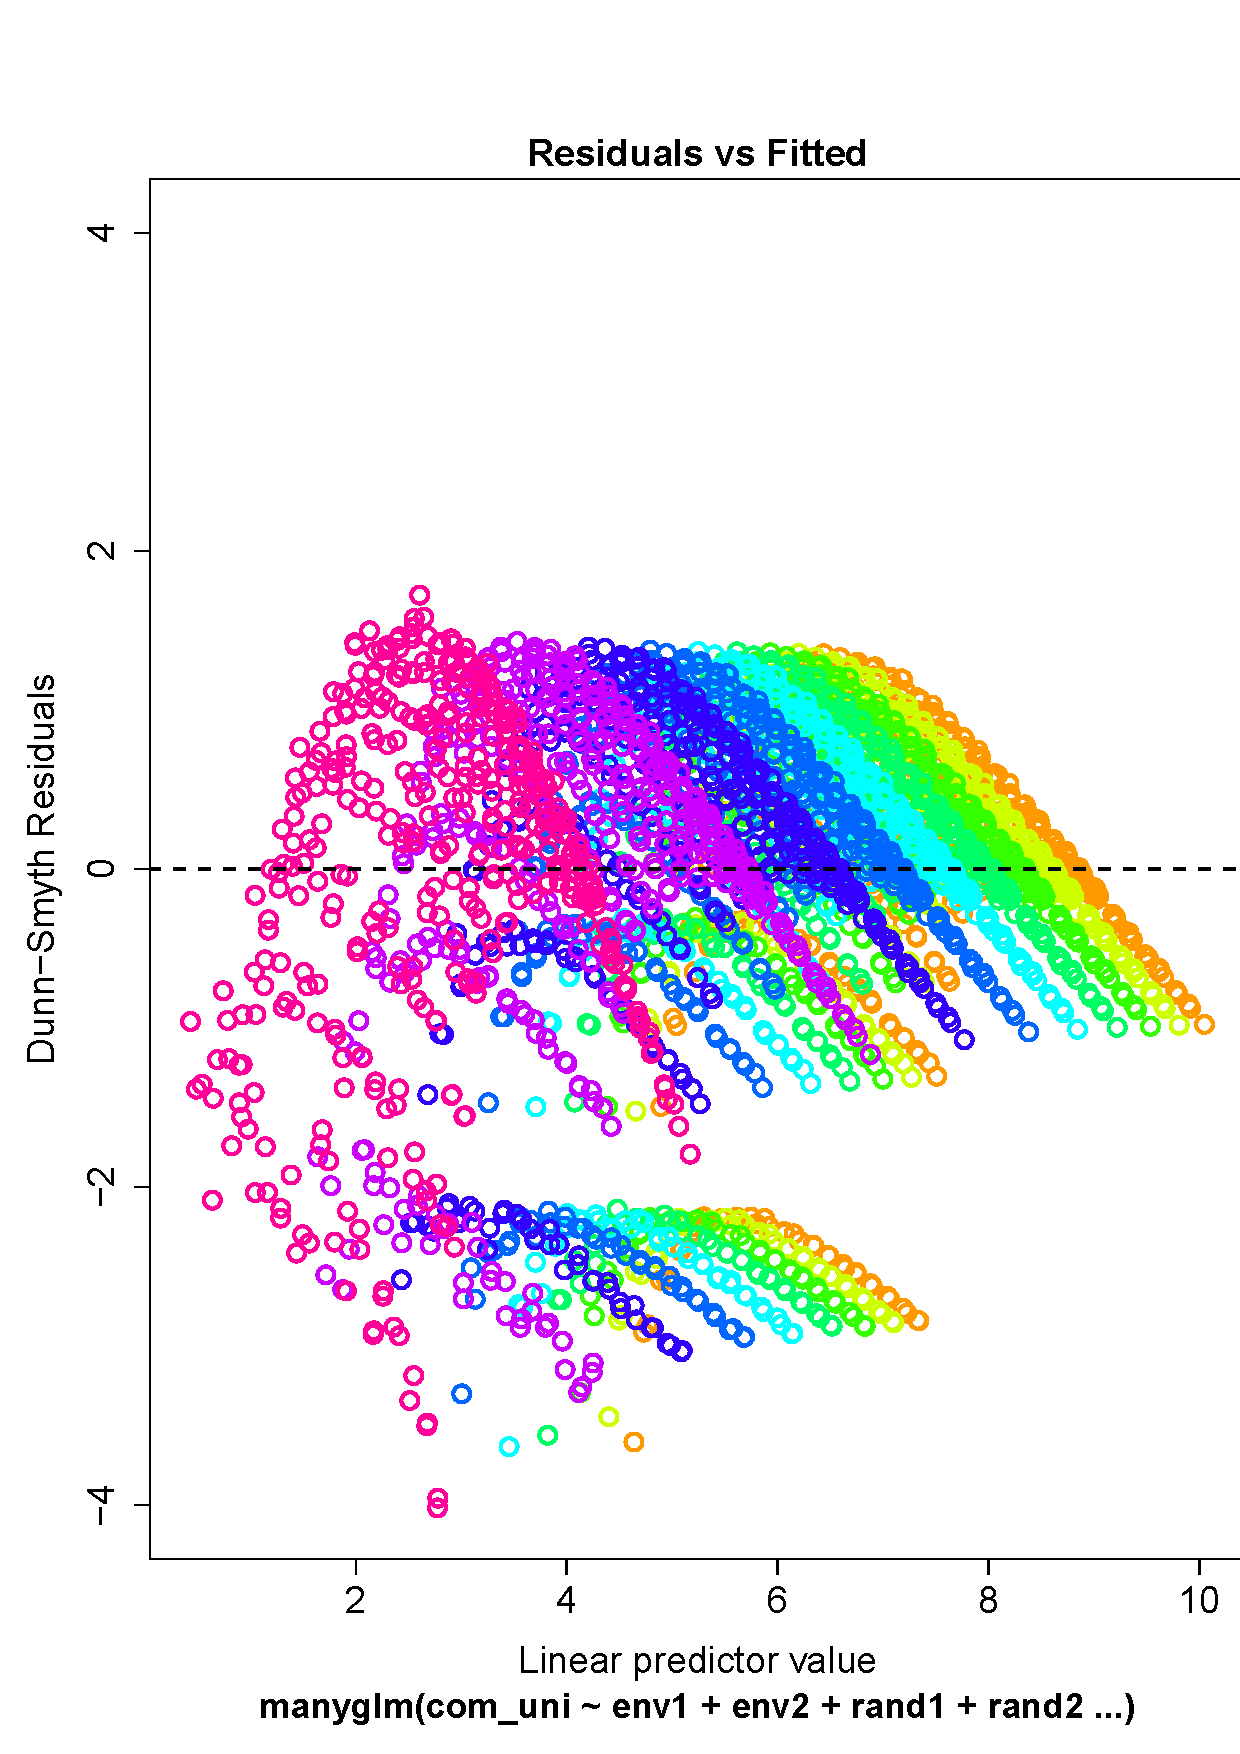
\includegraphics[scale = 0.4]{Arched_Dunn_Smyth}
%         \caption{The Dunn-Smyth residuals of the \textit{LL} community sampled with 400 samples plotted against the linear predictor. A pronounced arched pattern can be observed for every single species (different colors).}
%         \label{fig:arched_DS}
%     \end{figure}{}
    
  
    
%     \begin{figure}[!htbp]
%         \centering
%         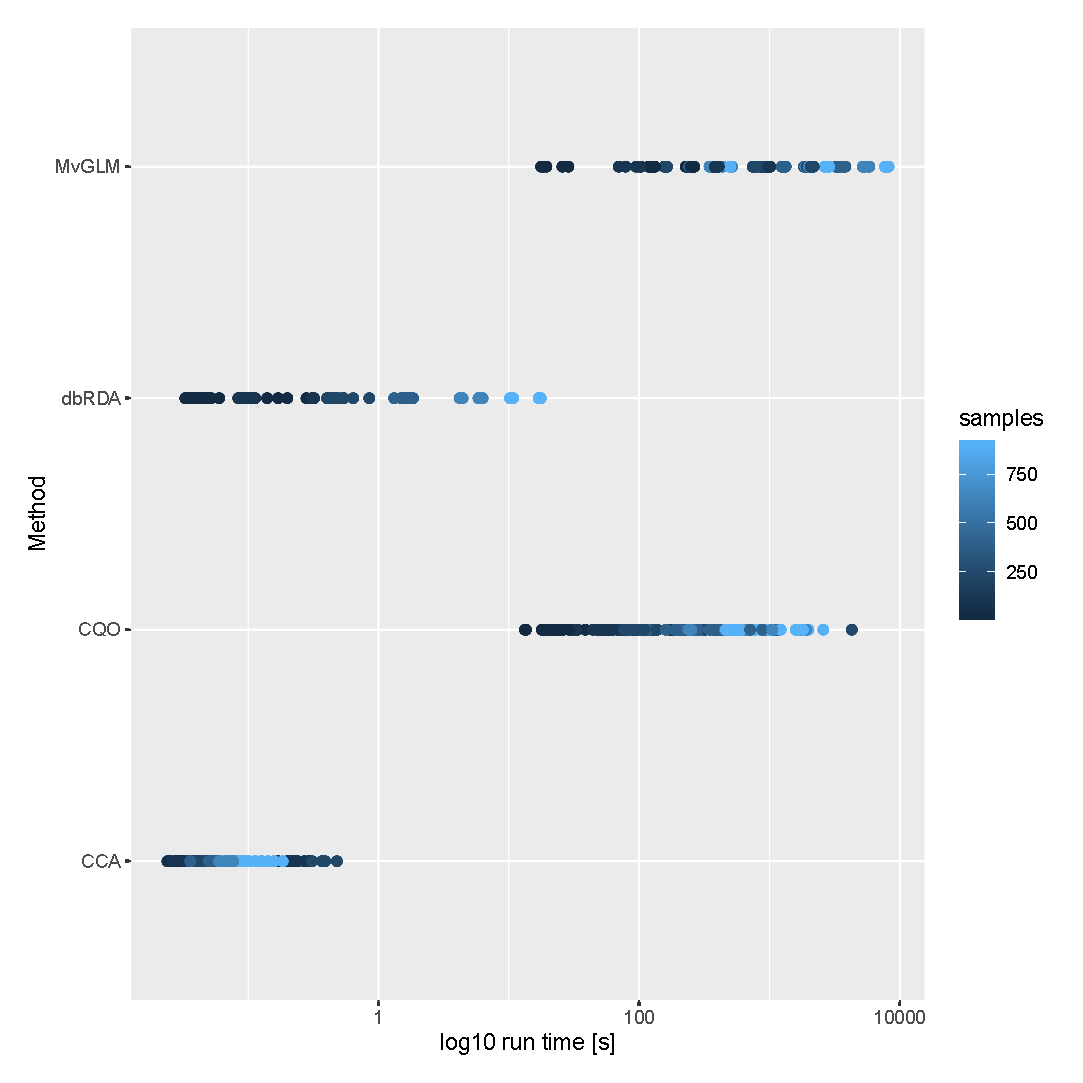
\includegraphics[scale =0.6]{runtimeplot}
%         \caption{
%         Run times of Multivariate Generalized Linear Models (MvGLM), distance-based Redundancy Analysis (dbRDA), Constrained Quadratic Ordination (CQO), and Canonical Correspondence Analysis (CCA). X-axis is scaled with a decimal logarithm. Colors indicate sample sizes.
%         }
%         \label{fig:runtime}
%     \end{figure}{}

% % 	Mean run time of CCA was below one second (s) and that of dbRDA was 4.3 s. 
% % 	%
% % 	There were no significant differences between different response types or sample sizes. 
% % 	%
% % 	CQO was the faster model-based method with a mean run time of 365 s.
% % 	%
% % 	Between response types, speed differed from 175 s (\textit{LL}) to 592 s (\textit{UB}). 
% % 	%
% % 	Mean run time increased linearly with sample size form 27 s (n = 25) to  972 s (n = 900).
% % 	%
% % 	MvGLM was the slowest method with a mean run time of 2159 s.
% % 	%
% % 	Again speed differed between response types and again \textit{LL} was the fastest with  741 s while \textit{BB} was the slowest with a mean run time of 3337 s.
% % 	%
% % 	Here too, run time increased linearly with samples size form 174 s (n = 25) to 5055 s (n = 900).
% % 	%
% % 	Note, however, that the times for CQO do not include the calculation of p-values which is quite time-consuming. 
% % \section{Further Result Statistics}	

% % page break 		
% 	\newpage	
% % 		This section contains all the mean \textit{p}-values at the level of response types or sample sizes.\\
% % 		%
% % 		Tables \ref{tab:mvglm:ss} and \ref{tab:mvglm:rs} show the mean \textit{p}-values of MvGLMs. 
% % 		%
% % 		% ------------------------------------------ %
% % 		%& TABLE: GLM multivariate p-Value of Classes
% % 		% ------------------------------------------- %
% \begin{table}[!htbp] 
%     \centering 
%     \caption{
%     Mean \textit{p}-values of Multivariate Generalized Linear Models with standard deviations for combinations of sample size and response type.
%     } 
%   \label{mvglm_sm_table} 
%     \begin{tabular}{@{\extracolsep{5pt}} cccccccc} 
%     \\[-1.8ex]\hline 
%     \hline \\[-1.8ex] 
%     && \multicolumn{2}{c}{env1} & \multicolumn{2}{c}{env2} & \multicolumn{2}{c}{Noise}\\\cmidrule(l){3-4} \cmidrule(l){5-6} \cmidrule(l){7-8}
%     %
%     && $\mu$ & $\sigma$ & $\mu$ & $\sigma$ & $\mu$ & $\sigma$\\ 
%     \hline \\[-1.8ex] 
%     UU & $25$ & $0.002$ & $0.001$ & $0.016$ & $0.005$ & $0.342$ & $0.228$ \\ 
%     UU & $100$ & $0.001$ & $0$ & $0.001$ & $0$ & $0.612$ & $0.267$ \\ 
%     UU & $225$ & $0.001$ & $0$ & $0.001$ & $0$ & $0.697$ & $0.265$ \\ 
%     UU & $400$ & $0.001$ & $0$ & $0.001$ & $0$ & $0.849$ & $0.129$ \\ 
%     UU & $625$ & $0.001$ & $0$ & $0.001$ & $0$ & $0.875$ & $0.138$ \\ 
%     UU & $900$ & $0.001$ & $0$ & $0.001$ & $0$ & $0.801$ & $0.219$ \\ 
%     UL & $25$ & $0.001$ & $0$ & $0.146$ & $0.007$ & $0.781$ & $0.162$ \\ 
%     UL & $100$ & $0.001$ & $0$ & $0.001$ & $0$ & $0.738$ & $0.210$ \\ 
%     UL & $225$ & $0.001$ & $0$ & $0.001$ & $0$ & $0.727$ & $0.283$ \\ 
%     UL & $400$ & $0.001$ & $0$ & $0.001$ & $0$ & $0.729$ & $0.258$ \\ 
%     UL & $625$ & $0.001$ & $0$ & $0.001$ & $0$ & $0.642$ & $0.250$ \\ 
%     UL & $900$ & $0.001$ & $0$ & $0.001$ & $0$ & $0.645$ & $0.272$ \\ 
%     UB & $25$ & $0.022$ & $0.003$ & $0.125$ & $0.010$ & $0.477$ & $0.256$ \\ 
%     UB & $100$ & $0.001$ & $0$ & $0.001$ & $0$ & $0.596$ & $0.264$ \\ 
%     UB & $225$ & $0.001$ & $0$ & $0.001$ & $0$ & $0.737$ & $0.224$ \\ 
%     UB & $400$ & $0.001$ & $0$ & $0.001$ & $0$ & $0.788$ & $0.171$ \\ 
%     UB & $625$ & $0.001$ & $0$ & $0.001$ & $0$ & $0.784$ & $0.249$ \\ 
%     UB & $900$ & $0.001$ & $0$ & $0.001$ & $0$ & $0.811$ & $0.170$ \\ 
%     LL & $25$ & $0.001$ & $0.0004$ & $0.001$ & $0$ & $0.406$ & $0.192$ \\ 
%     LL & $100$ & $0.001$ & $0$ & $0.001$ & $0$ & $0.587$ & $0.277$ \\ 
%     LL & $225$ & $0.001$ & $0$ & $0.001$ & $0$ & $0.514$ & $0.301$ \\ 
%     LL & $400$ & $0.001$ & $0$ & $0.001$ & $0$ & $0.574$ & $0.338$ \\ 
%     LL & $625$ & $0.001$ & $0$ & $0.001$ & $0$ & $0.593$ & $0.319$ \\ 
%     LL & $900$ & $0.001$ & $0$ & $0.001$ & $0$ & $0.460$ & $0.301$ \\ 
%     LB & $25$ & $0.166$ & $0.010$ & $0.001$ & $0$ & $0.776$ & $0.162$ \\ 
%     LB & $100$ & $0.001$ & $0$ & $0.001$ & $0$ & $0.717$ & $0.222$ \\ 
%     LB & $225$ & $0.001$ & $0$ & $0.001$ & $0$ & $0.736$ & $0.285$ \\ 
%     LB & $400$ & $0.001$ & $0$ & $0.001$ & $0$ & $0.721$ & $0.257$ \\ 
%     LB & $625$ & $0.001$ & $0$ & $0.001$ & $0$ & $0.639$ & $0.269$ \\ 
%     LB & $900$ & $0.001$ & $0$ & $0.001$ & $0$ & $0.643$ & $0.275$ \\ 
%     BB & $25$ & $0.001$ & $0$ & $0.010$ & $0.002$ & $0.363$ & $0.242$ \\ 
%     BB & $100$ & $0.001$ & $0$ & $0.001$ & $0$ & $0.432$ & $0.230$ \\ 
%     BB & $225$ & $0.001$ & $0$ & $0.001$ & $0$ & $0.618$ & $0.276$ \\ 
%     BB & $400$ & $0.001$ & $0$ & $0.001$ & $0$ & $0.828$ & $0.158$ \\ 
%     BB & $625$ & $0.001$ & $0$ & $0.001$ & $0$ & $0.814$ & $0.191$ \\ 
%     BB & $900$ & $0.001$ & $0$ & $0.001$ & $0$ & $0.717$ & $0.222$ \\ 
%     \hline \\[-1.8ex] 
%     \end{tabular} 
%     \end{table} 

% % page break 		
% 	\newpage	
	
% 	 %% -- CQO -- %% 
	 
% 	\begin{table}[!htbp] \centering 
%         \caption{
%             Mean \textit{p}-values of Constrained Quadratic Ordination with standard deviations for combinations of sample size and response type.
%         } 
%         \label{cqo_sm_table} 
%         \begin{tabular}{@{\extracolsep{5pt}} cccccccc} 
%             \\[-1.8ex]\hline 
%             \hline \\[-1.8ex] 
%             && \multicolumn{2}{c}{env1} & \multicolumn{2}{c}{env2} & \multicolumn{2}{c}{Noise}\\\cmidrule(l){3-4} \cmidrule(l){5-6} \cmidrule(l){7-8}
%             %
%             && $\mu$ & $\sigma$ & $\mu$ & $\sigma$ & $\mu$ & $\sigma$\\ 
%             \hline \\[-1.8ex] 
%             UU & $25$ & $0$ & $0$ & $0$ & $0$ & $0.820$ & $0.105$ \\ 
%             UU & $100$ & $0$ & $0$ & $0$ & $0$ & $0.879$ & $0.082$ \\ 
%             UU & $225$ & $0$ & $0$ & $0$ & $0$ & $0.875$ & $0.126$ \\ 
%             UU & $400$ & $0$ & $0$ & $0$ & $0$ & $0.917$ & $0.052$ \\ 
%             UU & $625$ & $0$ & $0$ & $0$ & $0$ & $0.880$ & $0.134$ \\ 
%             UU & $900$ & $0$ & $0$ & $0$ & $0$ & $0.952$ & $0.050$ \\ 
%             UL & $25$ & $0.127$ & $0.158$ & $0.289$ & $0.183$ & $0.646$ & $0.146$ \\ 
%             UL & $100$ & $0.071$ & $0.098$ & $0.240$ & $0.258$ & $0.612$ & $0.267$ \\ 
%             UL & $225$ & $0.004$ & $0.005$ & $0.010$ & $0.012$ & $0.506$ & $0.298$ \\ 
%             UL & $400$ & $0.006$ & $0.013$ & $0.087$ & $0.168$ & $0.569$ & $0.196$ \\ 
%             UL & $625$ & $0$ & $0$ & $0.519$ & $0.269$ & $0.990$ & $0$ \\ 
%             UL & $900$ & $0.008$ & $0.018$ & $0.705$ & $0.401$ & $0.990$ & $0$ \\ 
%             UB & $100$ & $0.024$ & $0.023$ & $0.026$ & $0.026$ & $0.654$ & $0.270$ \\ 
%             UB & $225$ & $0.026$ & $0.058$ & $0.014$ & $0.031$ & $0.702$ & $0.206$ \\ 
%             UB & $400$ & $0.036$ & $0.060$ & $0.002$ & $0.004$ & $0.658$ & $0.274$ \\ 
%             UB & $625$ & $0.010$ & $0.022$ & $0.020$ & $0.044$ & $0.583$ & $0.385$ \\ 
%             UB & $900$ & $0$ & $0$ & $0$ & $0$ & $0.639$ & $0.337$ \\ 
%             LL & $25$ & $0.085$ & $0.048$ & $0.143$ & $0.090$ & $0.400$ & $0.183$ \\ 
%             LL & $100$ & $0.154$ & $0.117$ & $0.095$ & $0.062$ & $0.723$ & $0.176$ \\ 
%             LL & $225$ & $0.091$ & $0.075$ & $0.081$ & $0.060$ & $0.841$ & $0.102$ \\ 
%             LL & $400$ & $0.180$ & $0.137$ & $0.263$ & $0.227$ & $0.761$ & $0.191$ \\ 
%             LL & $625$ & $0.281$ & $0.201$ & $0.208$ & $0.191$ & $0.779$ & $0.126$ \\ 
%             LL & $900$ & $0.295$ & $0.099$ & $0.188$ & $0.146$ & $0.838$ & $0.116$ \\ 
%             LB & $25$ & $0.265$ & $0.127$ & $0.141$ & $0.159$ & $0.619$ & $0.158$ \\ 
%             LB & $100$ & $0.097$ & $0.090$ & $0.038$ & $0.058$ & $0.619$ & $0.278$ \\ 
%             LB & $225$ & $0.067$ & $0.109$ & $0.006$ & $0.013$ & $0.589$ & $0.272$ \\ 
%             LB & $400$ & $0.174$ & $0.237$ & $0.006$ & $0.009$ & $0.586$ & $0.240$ \\ 
%             LB & $625$ & $0.204$ & $0.166$ & $0.044$ & $0.061$ & $0.504$ & $0.260$ \\ 
%             LB & $900$ & $0.164$ & $0.314$ & $0.020$ & $0.028$ & $0.561$ & $0.218$ \\ 
%             BB & $25$ & $0$ & $0$ & $0$ & $0$ & $0.591$ & $0.233$ \\ 
%             BB & $100$ & $0$ & $0$ & $0$ & $0$ & $0.359$ & $0.272$ \\ 
%             BB & $225$ & $0$ & $0$ & $0$ & $0$ & $0.573$ & $0.299$ \\ 
%             BB & $400$ & $0$ & $0$ & $0$ & $0$ & $0.636$ & $0.317$ \\ 
%             BB & $625$ & $0$ & $0$ & $0$ & $0$ & $0.421$ & $0.271$ \\ 
%             BB & $900$ & $0$ & $0$ & $0$ & $0$ & $0.543$ & $0.353$ \\ 
%             \hline \\[-1.8ex] 
%         \end{tabular} 
%     \end{table}
	
% % page break 		
% 	\newpage		
	
%     %% -- CCA -- %% 
%     \begin{table}[!htbp] \centering 
%         \caption{
%             Mean \textit{p}-values of Canonical Correspondence Analysis with standard deviations for combinations of sample size and response type.
%         } 
%         \label{cca_sm_table} 
%         \begin{tabular}{@{\extracolsep{5pt}} cccccccc} 
%             \\[-1.8ex]\hline 
%             \hline \\[-1.8ex] 
%             && \multicolumn{2}{c}{env1} & \multicolumn{2}{c}{env2} & \multicolumn{2}{c}{Noise}\\\cmidrule(l){3-4} \cmidrule(l){5-6} \cmidrule(l){7-8}
%             %
%             && $\mu$ & $\sigma$ & $\mu$ & $\sigma$ & $\mu$ & $\sigma$\\ 
%             \hline \\[-1.8ex] 
%             UU & $25$ & $0.001$ & $0$ & $0.001$ & $0$ & $0.001$ & $0$ \\ 
%             UU & $100$ & $0.001$ & $0$ & $0.001$ & $0$ & $0.467$ & $0.355$ \\ 
%             UU & $225$ & $0.001$ & $0$ & $0.001$ & $0$ & $0.093$ & $0.113$ \\ 
%             UU & $400$ & $0.001$ & $0$ & $0.001$ & $0$ & $0.349$ & $0.336$ \\ 
%             UU & $625$ & $0.001$ & $0$ & $0.001$ & $0$ & $0.153$ & $0.275$ \\ 
%             UU & $900$ & $0.001$ & $0$ & $0.001$ & $0$ & $0.247$ & $0.362$ \\ 
%             UL & $25$ & $0.001$ & $0$ & $0.987$ & $0.014$ & $0.403$ & $0.288$ \\ 
%             UL & $100$ & $0.001$ & $0$ & $1$ & $0$ & $0.329$ & $0.294$ \\ 
%             UL & $225$ & $0.001$ & $0$ & $1$ & $0$ & $0.346$ & $0.274$ \\ 
%             UL & $400$ & $0.001$ & $0$ & $1$ & $0$ & $0.393$ & $0.317$ \\ 
%             UL & $625$ & $0.001$ & $0$ & $1$ & $0$ & $0.436$ & $0.219$ \\ 
%             UL & $900$ & $0.001$ & $0$ & $1$ & $0$ & $0.439$ & $0.321$ \\ 
%             UB & $25$ & $0.001$ & $0$ & $0.001$ & $0$ & $0.035$ & $0.074$ \\ 
%             UB & $100$ & $0.001$ & $0$ & $0.001$ & $0$ & $0.344$ & $0.269$ \\ 
%             UB & $225$ & $0.001$ & $0$ & $0.001$ & $0$ & $0.244$ & $0.283$ \\ 
%             UB & $400$ & $0.001$ & $0$ & $0.001$ & $0$ & $0.172$ & $0.195$ \\ 
%             UB & $625$ & $0.001$ & $0$ & $0.001$ & $0$ & $0.111$ & $0.192$ \\ 
%             UB & $900$ & $0.001$ & $0$ & $0.001$ & $0$ & $0.066$ & $0.170$ \\ 
%             LL & $25$ & $0.992$ & $0.012$ & $0.997$ & $0.005$ & $0.976$ & $0.031$ \\ 
%             LL & $100$ & $0.985$ & $0.009$ & $0.989$ & $0.005$ & $0.994$ & $0.011$ \\ 
%             LL & $225$ & $0.712$ & $0.046$ & $0.691$ & $0.031$ & $0.962$ & $0.069$ \\ 
%             LB & $25$ & $0.987$ & $0.015$ & $0.001$ & $0$ & $0.398$ & $0.289$ \\ 
%             LB & $100$ & $1$ & $0$ & $0.001$ & $0$ & $0.358$ & $0.307$ \\ 
%             LB & $225$ & $1$ & $0$ & $0.001$ & $0$ & $0.378$ & $0.278$ \\ 
%             LB & $400$ & $1$ & $0$ & $0.001$ & $0$ & $0.412$ & $0.331$ \\ 
%             LB & $625$ & $1$ & $0$ & $0.001$ & $0$ & $0.438$ & $0.209$ \\ 
%             LB & $900$ & $1$ & $0$ & $0.001$ & $0$ & $0.446$ & $0.321$ \\ 
%             BB & $25$ & $0.001$ & $0$ & $0.001$ & $0$ & $0.564$ & $0.286$ \\ 
%             BB & $100$ & $0.001$ & $0$ & $0.001$ & $0$ & $0.469$ & $0.341$ \\ 
%             BB & $225$ & $0.001$ & $0$ & $0.001$ & $0$ & $0.580$ & $0.301$ \\ 
%             BB & $400$ & $0.001$ & $0$ & $0.001$ & $0$ & $0.566$ & $0.314$ \\ 
%             BB & $625$ & $0.001$ & $0$ & $0.001$ & $0$ & $0.497$ & $0.343$ \\ 
%             BB & $900$ & $0.001$ & $0$ & $0.001$ & $0$ & $0.491$ & $0.330$ \\ 
%             \hline \\[-1.8ex] 
%         \end{tabular} 
%     \end{table}
% % page break 		
% 	\newpage		
	
%     %% -- dbRDA -- %% 
%     \begin{table}[!htbp] \centering 
%         \caption{
%             Mean \textit{p}-values of distance-based Redundancy Analysis with standard deviations for combinations of sample size and response type.
%         } 
%         \label{dbrda_sm_table} 
%         \begin{tabular}{@{\extracolsep{5pt}} cccccccc} 
%             \\[-1.8ex]\hline 
%             \hline \\[-1.8ex] 
%             && \multicolumn{2}{c}{env1} & \multicolumn{2}{c}{env2} & \multicolumn{2}{c}{Noise}\\\cmidrule(l){3-4} \cmidrule(l){5-6} \cmidrule(l){7-8}
%             %
%             && $\mu$ & $\sigma$ & $\mu$ & $\sigma$ & $\mu$ & $\sigma$\\ 
%             \hline \\[-1.8ex] 
%             UU & $25$ & $0.001$ & $0$ & $0.001$ & $0$ & $0.510$ & $0.302$ \\ 
%             UU & $100$ & $0.001$ & $0$ & $0.001$ & $0$ & $0.669$ & $0.304$ \\ 
%             UU & $225$ & $0.001$ & $0$ & $0.001$ & $0$ & $0.457$ & $0.238$ \\ 
%             UU & $400$ & $0.001$ & $0$ & $0.001$ & $0$ & $0.611$ & $0.275$ \\ 
%             UU & $625$ & $0.001$ & $0$ & $0.001$ & $0$ & $0.561$ & $0.173$ \\ 
%             UU & $900$ & $0.001$ & $0$ & $0.001$ & $0$ & $0.451$ & $0.275$ \\ 
%             UL & $25$ & $0.001$ & $0$ & $0.066$ & $0.010$ & $0.553$ & $0.240$ \\ 
%             UL & $100$ & $0.001$ & $0$ & $0.001$ & $0$ & $0.517$ & $0.275$ \\ 
%             UL & $225$ & $0.001$ & $0$ & $0.001$ & $0$ & $0.470$ & $0.268$ \\ 
%             UL & $400$ & $0.001$ & $0$ & $0.001$ & $0$ & $0.581$ & $0.278$ \\ 
%             UL & $625$ & $0.001$ & $0$ & $0.001$ & $0$ & $0.529$ & $0.199$ \\ 
%             UL & $900$ & $0.001$ & $0$ & $0.001$ & $0$ & $0.437$ & $0.228$ \\ 
%             UB & $25$ & $0.001$ & $0$ & $0.001$ & $0$ & $0.486$ & $0.291$ \\ 
%             UB & $100$ & $0.001$ & $0$ & $0.001$ & $0$ & $0.712$ & $0.245$ \\ 
%             UB & $225$ & $0.001$ & $0$ & $0.001$ & $0$ & $0.435$ & $0.235$ \\ 
%             UB & $400$ & $0.001$ & $0$ & $0.001$ & $0$ & $0.629$ & $0.234$ \\ 
%             UB & $625$ & $0.001$ & $0$ & $0.001$ & $0$ & $0.591$ & $0.119$ \\ 
%             UB & $900$ & $0.001$ & $0$ & $0.001$ & $0$ & $0.424$ & $0.272$ \\ 
%             LL & $25$ & $0.010$ & $0.005$ & $0.009$ & $0.007$ & $0.520$ & $0.219$ \\ 
%             LL & $100$ & $0.001$ & $0$ & $0.001$ & $0$ & $0.467$ & $0.261$ \\ 
%             LL & $225$ & $0.001$ & $0$ & $0.001$ & $0$ & $0.477$ & $0.261$ \\ 
%             LL & $400$ & $0.001$ & $0$ & $0.001$ & $0$ & $0.665$ & $0.293$ \\ 
%             LL & $625$ & $0.001$ & $0$ & $0.001$ & $0$ & $0.589$ & $0.290$ \\ 
%             LL & $900$ & $0.001$ & $0$ & $0.001$ & $0$ & $0.347$ & $0.298$ \\ 
%             LB & $25$ & $0.044$ & $0.008$ & $0.001$ & $0$ & $0.550$ & $0.241$ \\ 
%             LB & $100$ & $0.001$ & $0$ & $0.001$ & $0$ & $0.514$ & $0.277$ \\ 
%             LB & $225$ & $0.001$ & $0$ & $0.001$ & $0$ & $0.473$ & $0.266$ \\ 
%             LB & $400$ & $0.001$ & $0$ & $0.001$ & $0$ & $0.584$ & $0.276$ \\ 
%             LB & $625$ & $0.001$ & $0$ & $0.001$ & $0$ & $0.521$ & $0.194$ \\ 
%             LB & $900$ & $0.001$ & $0$ & $0.001$ & $0$ & $0.437$ & $0.224$ \\ 
%             BB & $25$ & $0.001$ & $0$ & $0.001$ & $0$ & $0.564$ & $0.296$ \\ 
%             BB & $100$ & $0.001$ & $0$ & $0.001$ & $0$ & $0.572$ & $0.316$ \\ 
%             BB & $225$ & $0.001$ & $0$ & $0.001$ & $0$ & $0.496$ & $0.258$ \\ 
%             BB & $400$ & $0.001$ & $0$ & $0.001$ & $0$ & $0.481$ & $0.195$ \\ 
%             BB & $625$ & $0.001$ & $0$ & $0.001$ & $0$ & $0.466$ & $0.237$ \\ 
%             BB & $900$ & $0.001$ & $0$ & $0.001$ & $0$ & $0.467$ & $0.265$ \\ 
%             \hline \\[-1.8ex] 
%         \end{tabular} 
%     \end{table}
\end{document}
